% !TeX spellcheck = es_ES
\documentclass{article}


\usepackage[utf8]{inputenc}

\usepackage{amssymb}


%\usepackage[pdftex]{graphicx}
\usepackage{amsfonts}
\usepackage{amssymb}
\usepackage{amsmath}
\usepackage{mathtools}
\usepackage{listings}
\usepackage{caption}
\usepackage{graphicx}
\usepackage{float}

\usepackage[backend=bibtex,style=numeric]{biblatex}
\usepackage[titletoc]{appendix}
\addbibresource{doc.bib}
\usepackage{hyperref}
\hypersetup{
	colorlinks,
	citecolor=black,
	filecolor=black,
	linkcolor=black,
	urlcolor=black
}

\usepackage{amsthm}

\renewcommand{\contentsname}{Índice}
\renewcommand\appendixtocname{Apéndice}
\renewcommand{\figurename}{Figura}
\usepackage{etoolbox}
\renewcommand*{\proofname}{Prueba}

\newtheorem{theorem}{Teorema}


\begin{document}
	\begin{titlepage}
		
		\vspace*{\fill}
		\begin{center}
			
			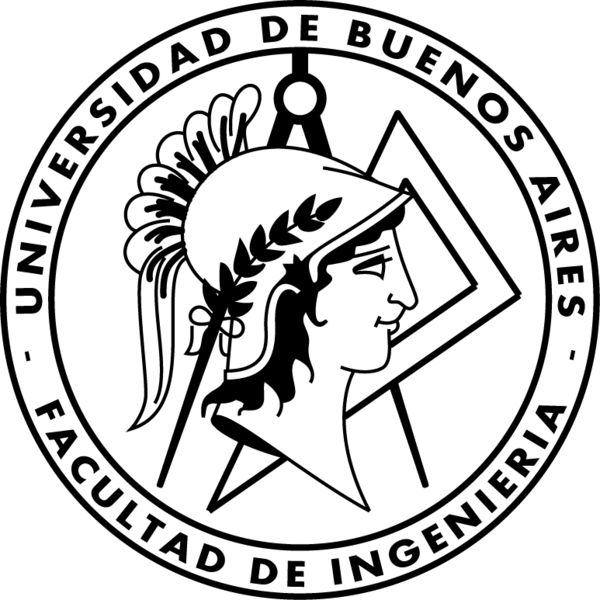
\includegraphics[scale=1]{fiuba.png}\\
			\quad\linebreak
			\quad\linebreak
			\huge Exploración de celdas LSTM iterativas como método de inferencia incremental.
			\quad\linebreak
			
			\quad\linebreak
			\large \textbf{Leandro Palma}\\
			\quad\linebreak	
			\quad\linebreak
			\textit{En cumplimiento de los requerimientos para obtener el título de\\
				Ingeniero en Informática}\\
			\quad\linebreak
			\quad\linebreak
			Director: Lic. Luis Argerich\\
			
			\quad\linebreak
			\quad\linebreak
			Departamento de Computación\\
			
			Facultad de Ingeniería\\
			
			Universidad de Buenos Aires\\
			
			2018
		\end{center}
		
		\vspace*{\fill}
	\end{titlepage}
	
	\pagebreak
	\vspace*{\fill}
	
	\begin{center}
		\Large\textbf{Resumen}
		\quad\linebreak
		
		
		\normalsize
	\end{center}	
	\normalsize
	
	Las RNNs han sido ampliamente difundidas y en la actualidad se aplican sobre modelos de secuencia en diversas tareas en el campo de machine learning e inteligencia artificial. El estudio de estas redes ha sido enfocado en la explotación de su capacidad para mejorar el desempeño de modelos que representan procesos secuenciales. Sin embargo, poco se ha innovado sobre la estructura recurrente de estas redes más allá de soluciones a problemas específicos como el conocido problema del desvanecimiento y la saturación del gradiente.\\
	La presente investigación analiza las celdas LSTM desde la perspectiva del estudio de sistemas dinámicos para proponer una modificación sobre el flujo de información en la misma. Se presenta una implementación\footnote{\texttt{https://github.com/PalmaLeandro/iterativeLSTM}\label{footnote1}} de la modificación propuesta y se realizan experimentos sobre la tarea de modelado del lenguaje obteniendo un desempeño comparable con conocidos modelos más complejos en términos de cantidad de parámetros.\\
	Los modelos neuronales recurrentes que aplican la modificación propuesta mejoran consistentemente su desempeño obteniendo una perplejidad similar para modelos del lenguaje con una reducción mayor al \%300 en la cantidad de parámetros respecto de sus versiones originales.\\
	\textbf{Palabras clave:} sistemas dinámicos, RNNs, celdas LSTM, modelado del lenguaje.\\
	
	
	\vspace*{\fill}
	\pagebreak
	\vspace*{\fill}
	\begin{center}
		\Large\textbf{Abstract}\\
	\end{center}	
	\normalsize
	RNNs have been widely diffused and today they are used over a vast number of sequence models applied to diverse tasks on the field of machine learning and artificial intelligence. The study of such networks has been focused on the exploration of its capabilities to improve the performance of models that represent sequential processes. However, there has been little innovation in respect to the recurrent structure of such networks other than solutions to specific issues, such as the gradient vanish and gradient exploding problems. \\
	The present research analyses the LSTM cells from the perspective of the study of dynamic systems in order to propose a modification over the information flow in it. The implementation of such modification is presented in this work with experiments performed over the language modeling task achieving performance comparable to more complex well-known models in terms of number of parameters.\\
	The recurrent neural models that apply the proposed modification consistently improve their performance achieving a similar perplexity for language models with a reduction over \%300 in the number of parameters with respect to their original models.\\
	\textbf{Keywords:} dynamic systems, RNNs, LSTM cells, language modeling.\\
	
	\vspace*{\fill}
	\pagebreak
	
	
	\tableofcontents
	
	\pagebreak
	\section{Introducción}\label{sectionIntroduction}
	
	
	Actualmente los modelos de secuencia, y particularmente las redes neuronales recurrentes(RNN), son ampliamente usados debido a su versatilidad para retener y procesar información sobre secuencias de datos con longitud variable, manteniendo las dependencias temporales entre los sucesivos eventos, tanto en el entrenamiento del modelo como en las predicciones realizadas por el mismo.\\
	A pesar de los múltiples esfuerzos realizados para mejorar su desempeño\cite{16ForgateGatePeepholeConnectionsGers} y de su innegable importancia en el desarrollo de modelos tanto académicos\cite{15TransductionGraves, 43ParsingScenesRecursively, 44SpeechRecognition, 52MachineTranslationAttentionRNN} como industriales\cite{12DeepSearch, 13SpeechRecognition, 14RegularizationZaremba, 51SequenceToSequenceMachineTranslation, 56MicrosoftSpeechRecognition}, la estructura básica de dichos modelos solo sufrió ligeras variaciones desde la publicación de las celdas Long Short-Term Memory(LSTM), hace poco más de 20 años\cite{42FormerLSTMHochreiter}. \\
	Motivados por los problemas de desvanecimiento de la señal de entrenamiento presentes en las RNN, los autores de las celdas LSTM propusieron modificaciones sobre la estructura de cada \textit{unit} con la finalidad de retener íntegramente las dependencias temporales en los datos procesados a partir de considerar el contexto en su evaluación y en la propagación de errores durante el entrenamiento\cite{42FormerLSTMHochreiter}.\\
	Estos problemas son comúnmente denominados \textit{``gradient vanish"}, para el caso del desvanecimiento de la señal, y  \textit{``gradient exploding"} para el caso de la saturación de la señal. Su solución que será explorada en la sección \ref{sectionLSTM} es relativamente sencilla e indudablemente eficaz.\\
	
	Sin embargo, existen potenciales inconvenientes en dicha solución relacionados con el mecanismo por el cual las RNNs retienen la información registrada. Su resolución ofrece apreciables mejoras en el desempeño del modelo que serán expuestas tanto experimentalmente como en forma teórica y, según me consta, no fueron abordadas por la literatura disponible en el campo hasta el momento de realizada esta investigación.\\
	Aprovechar todo el potencial de las RNNs requerirá su estudio desde la perspectiva de sistemas dinámicos, donde se encuentran explicaciones a la capacidad de estas redes para retener información y posibilidades de optimizar sus resultados en un esquema iterativo.\\
	Recientes publicaciones de nuevas arquitecturas de redes neuronales \cite{1GANs, 18DifferentiableNeuralComputer} fomentan el estudio de nuevas estructuras de redes neuronales que permitan extraer información de los datos secuenciales más eficazmente, reconociendo patrones incrementalmente más complejos.\\
	
	La presente investigación tiene como objetivo explorar cambios en el flujo de información a través de una capa de celdas LSTM realizando sucesivas iteraciones que evalúen la clasificación de cada celda sobre los mismos datos de entrada, alterando el estado de la red. \\
	La ejecución de las iteraciones es condicionada por una regresión logística sobre las variables internas de las celdas y el estado resultante de la misma.\\
	
	Los resultados hallados sobre los experimentos realizados en tareas del campo de procesamiento del lenguaje natural(NPL, por sus siglas en inglés) y en forma teórica sobre la teoría de sistemas dinámicos sugieren que el esquema propuesto permite explotar el potencial de las celdas LSTM más allá de su desempeño normal.
	
	\subsection{Trabajo Previo}
	La modificación propuesta sobre la estructura de la celda LSTM define un sistema dinámico, el cual evoluciona el vector de estado del bloque de celdas LSTM durante sucesivas iteraciones. \\
	En este escenario la evolución del estado individual de cada celda del bloque está acoplada a la evolución de los estados de las otras celdas del bloque a través de parámetros que ponderan las conexiones recurrentes. Esta propiedad asemeja la estructura que aplica la modificación propuesta con la variante de RNN, Echo State Network(ESN). Estos modelos emplean un reservorio constituido por una RNN cuyos parámetros han sido inicializados de forma aleatoria, pero limitados a un conjunto de valores que producen dependencias relevantes entre las celdas de la red.\\
	La arquitectura ESN es mayormente usada para predicción de series continuas de tiempo, por lo tanto, para frecuencias de muestreo sobre la secuencia de valores de entrada suficientemente altos como para considerar dichos valores constantes, se tiene un esquema similar al propuesto donde se realizan sucesivas evaluaciones de la RNN sobre los mismos valores de entrada.\\
	
	Recientemente en Laurent et.al(2016)\cite{11Laurent} se exploran distintas estructuras de RNNs desde la perspectiva del estudio de sistemas dinámicos buscando remediar el comportamiento caótico de dichos sistema bajo condiciones particulares. El extenso análisis presentado en dicha publicación difiere del análisis presentado en las condiciones bajo las que se estudia el sistema dinámico descrito por la evolución del estado de las RNNs. Adicionalmente, la motivación de dicho análisis es la de exponer el comportamiento de los sistemas mientras que el análisis presentado busca condiciones de la RNN para las cuales se obtiene el comportamiento convergente deseado.\\
	
	La modificación propuesta se relaciona con otras estructuras iterativas\cite{2BridgingGaps} de RNNs que evolucionan una representación intermedia entre sucesivas iteraciones con la motivación de inferir de forma incremental el resultado esperado. Sin embargo, estas estructuras no contemplan la dinámica descrita por la RNN para producir la convergencia del vector de estado y su consiguiente robustez para representar la información registrada.\\
	
	Un ejemplo de estructura iterativa de RNN existente es LoopyRNN\cite{17LoopyRNN}. Esta red recurrente realiza sucesivas iteraciones tomando como entradas el resultado previamente obtenido. Mientras este comportamiento es análogo al propuesto por la modificación sugerida, el mismo aplica el enfoque iterativo sobre el flujo que pondera los valores de las variables de entrada a la celda a diferencia de la evolución iterativa del estado de la celda propuesto. Se consideró el enfoque tomado en dicha investigación como precursor de la modificación propuesta en la que se contempló desde la perspectiva del estudio de los sistemas dinámicos que es el estado de la celda el que debería evolucionar guiado por la influencia del presente valor de las variables de entrada.\\
	Finalmente, el trabajo presentado contempla los efectos de la modificación propuesta sobre los conocidos problemas de entrenar RNNs para que extraer información de secuencias de eventos que presentan dependencias temporales separadas por largos intervalos de tiempo.
	
	\subsection{Organización}
	El resto del documento se organiza de la siguiente forma. 
	En la sección \ref{sectionRNN} se describe los fundamentos detrás de la estructura de una red neuronal recurrente, se introduce su estudio como un sistema dinámico y se exponen los problemas que motivaron el desarrollo de la celda LSTM. \\
	La sección \ref{sectionLSTM} describe las mejoras obtenidas con la estructura de las celdas LSTM original, explora diversas modificaciones propuestas sobre dicha estructura y las mejoras obtenidas en cada caso.\\
	La sección \ref{sectionIterativeLSTM} explica en detalle la mejora iterativa propuesta y los fundamentos teóricos detrás de su desempeño.\\
	La sección \ref{sectionLanguageModeling} detalla la aplicación de RNNs sobre la tarea de modelado del lenguaje.\\
	La sección \ref{sectionExperiments} expone de forma comparativa los resultados obtenidos con modelos que usan celdas LSTM tradicionales y modelos que usan celdas con la mejora iterativa propuesta en su aplicación al problema de modelado del lenguaje. \\
	Finalmente, en la sección \ref{sectionConclusions} resume las contribuciones del trabajo realizado y posibles aspectos a indagar como trabajo futuro.
	
	\subsection{Notación}
	Durante el desarrollo del presente documento se identificarán los siguientes elementos con su símbolo correspondiente:
	\begin{equation*}
	\begin{split}
	t, \; &\parbox[t]{32em}{ es el indice que indica un instante en una secuencia de valores ordenados.}\\
	\quad\\
	\tau, \; &\parbox[t]{32em}{ es el indice que indica el numero de iteración. \\
		Implica una escala de tiempo de menor orden que la escala de tiempo \textit{t}.\\
		Esta escala es intrínseca a un instante de tiempo \textit{t} y durante el resto del documento se referencia a la escala correspondiente un mismo instante \textit{t} genérico.}\\
	\quad\\
	h(t), \; &\parbox[t]{32em}{ es valor del vector de estado de la RNN al finalizar la evaluación correspondiente al instante \textit{t}.\\
		En el caso de la RNN que aplica la modificación propuesta este vector solo esta disponible al finalizar la última iteración.}\\
	\quad\\
	h(\tau), \; &\parbox[t]{32em}{ es un vector con los valores del estado de la RNN al finalizar la iteración $\tau$.}\\
	\quad\\
	x(t), \; &\parbox[t]{32em}{ es un vector con los valores de las variables de entrada de la RNN en el instante t de la secuencia.}\\
	\quad\\
	y(t), \; &\parbox[t]{32em}{ es el resultado de la evaluación de la RNN en el instante t.\\
		Forma el valor de la secuencia de salida en el instante t .}\\
	\quad\\
	\mathcal{E}(t), \; &\parbox[t]{32em}{ es el error en la clasificación y(t) respecto del valor esperado.\\
		La magnitud de este valor está dado por la función objetivo a usar para optimizar el conjunto de parametros $\theta$.}\\
	\quad\\
	\theta, \; &\parbox[t]{32em}{ es el conjunto de parámetros a optimizar presentes en el modelo usado para minimizar $\mathcal{E}(t)$.}\\
	\quad\\
	\end{split}
	\end{equation*}
	
	\pagebreak
	\section{RNNs}\label{sectionRNN}
	En esta sección se describe la formulación matemática de las RNN, se mencionan ejemplos de arquitecturas que emplean RNNs como mecanismo para procesar secuencias de eventos, además de presentar un análisis de las RNNs como sistemas dinámicos y finalmente exponer los problemas inherentes a su definición que motivaron el desarrollo de las celdas LSTM.\\
	Las RNN son modelos de secuencia que generalizan a las redes neuronales(NN) tradicionales\cite{19IntroductionRNN}. En las RNN el conjunto de parámetros $\theta$ es compartido durante los sucesivos instantes en los que se evalúa el modelo, aplicando una operación de clasificación no lineal en cada instante \textit{t} cuyo resultado varía según el valor de las variables de entrada y el estado \textit{h} del la red antes de realizar la clasificación.\\ 
	
	Formalmente, una RNN básica procesa una secuencia de valores de entrada \textit{$(x(1) , ... , x(T))$}, produciendo una secuencia de valores de salida \textit{ $(y(1), ... , y(T))$} a partir de aplicar sucesivamente y en forma ordenada las siguientes ecuaciones sobre cada instante de tiempo $t$ 
	\begin{equation}\label{RNN}
	h(t) = g( W_{in} x(t) + W_{rec} h(t-1) + b )
	\end{equation}
	\begin{equation*}
	y(t) = h(t)
	\end{equation*}
	
	Donde $h_{t}$ es el estado de la red inmediatamente después de realizar la clasificación. $g$ es una función diferenciable y continua aplicada a cada coeficiente del vector de entrada tal que $f: \mathbb{R} \rightarrow \mathbb{R}$, siendo normalmente seleccionada como la función tangente hiperbólica o la función sigmoidea pero pudiendo ser cualquier función diferenciable y continua que escale apropiadamente la entrada. \\
	Generalmente se considera la dificultad en el cálculo de la derivada de estas funciones para su selección debido a que las mismas deberán ser calculadas para cada celda a ser entrenada usando un método del gradiente.\\
	$W_{in}$, $W_{rec}$ son matrices que ponderan las variables de entrada y el estado previo de la red, y en conjunto con el vector de sesgos $b$ conforman el set de parámetros $\theta$ de la RNN. Los mismos son inicializados con valores aleatorios según una distribución uniforme $\theta \sim \mathcal{U}(-\sigma, \sigma)$ donde $\sigma$ es un parámetro a seleccionar por el usuario, normalmente tomado como $0.1$.\\
	
	La estructura de procesamiento de la RNN básica presentada es visible en la figura \ref{basicRNN}.
	\begin{figure}[H]
		\centering
		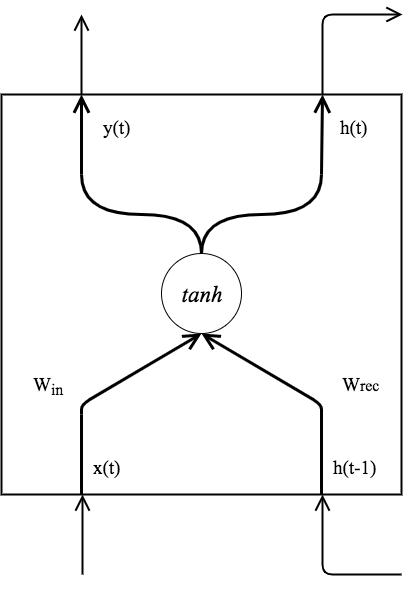
\includegraphics[scale=0.2]{basicRNN}
		\caption{Flujo de información en una RNN básica.}
		\label{basicRNN}
	\end{figure}
	
	Como es apreciable en la figura \ref{basicRNN}, una RNN básica realiza una clasificación a partir de exponer la activación de una función no lineal, típicamente $tanh(\cdot)$, sobre una regresión de los valores $x(t)$ de las variables entrada y el estado de la red $h(t-1)$ al momento de ser evaluada. En la sección \ref{sectionIterativeLSTM} exploraremos en detalle la dependencia con el estado de la celda para entender su participación en la clasificación realizada.\\
	
	En la definición dada en (\ref{RNN}) puede notarse la realimentación del estado previo $h(t-1)$ por el cual las RNNs mantienen la información registrada en los coeficientes del vector $h$ en forma \textit{``analógica"}, es decir, como un vector de valores continuos. Esta propiedad es necesaria para que el modelo represente al proceso de una forma diferenciable y continua sobre el espacio de parámetros $\mathbb{R}^{|\theta|}$, donde $|\theta|$ el número de parámetros del modelo. 
	De esta forma el conjunto de parámetros $\theta$ puede ser optimizado usando algoritmos que usen el gradiente de una función objetivo como señal de entrenamiento. \\
	Estos métodos se conocen como basados en el gradiente\cite{20SutskeverPhdThesis} e incluyen Backpropagation (BP) y su generalización sobre sucesivos instantes de tiempo, Backpropagation Through Time (BPTT) que actualmente constituye el método estándar de entrenamiento de RNNs.\\
	
	En la siguiente subsección se expone como la dinámica definida en (\ref{RNN}) le permite al modelo almacenar información en forma discreta, análogamente a como lo hace una computadora ordinaria usando bits. También se expondrá el problema inherente de las RNNs para procesar secuencias de amplia longitud siendo entrenadas por el método BPTT.\\
	
	Dependiendo del proceso estocástico que se modele y que es propio de la tarea a resolver, la arquitectura de la red puede variar. Posibles cambios al modelo incluyen la agregar más \textit{capas} en la RNN, cuya dinámica será similar a la de la RNN anteriormente definida pero tomarán como entradas las representaciones de las capas inferiores. De esta forma se generan representaciones internas de las variables de entrada\cite{5IntermediateFeatures} que sean de interés para la tarea a resolver.\\
	En términos generales, la ventaja de disponer de un mayor número de capas radica en que es posible obtener clasificaciones más complejas sobre las variables de la secuencia de entrada.\\ Adicionalmente, aumentar las capas de la red implica aumentar el número de parámetros del modelo aumentando también la dificultad de evitar el problema de \textit{overfitting}. Este problema se materializa cuando la optimización del conjunto de parámetros $\theta$ sobre el conjunto de datos de entrenamiento resulta en soluciones que tienen un muy buen desempeño sobre las secuencias de dicho conjunto pero un desempeño muy malo sobre secuencias que no estuvieran presentes en dicho conjunto.\\
	El problema subyacente a la carencia de desempeño sobre secuencias desconocidas para el modelo es la falta de \textit{generalización} sobre las secuencias del set de entrenamiento. En este caso el desempeño óptimo sobre el conjunto de secuencias de entrenamiento se debe a que el modelo memoriza las salidas correspondientes a cada secuencia de entrada.\\
	El estudio de la generalización de los modelos es un tópico muy estudiado en el campo de machine learning y en este trabajo se comentan únicamente los efectos más comunes sobre la arquitectura elegida. Para un completo estudio completo del problema de generalización se refiere al lector a Zhang et.al(2016)\cite{6Generalization}.\\
	
	Otros aspectos a considerar son la complejidad del cálculo de la inferencia del modelo, el tiempo de procesamiento y la cantidad de memoria requerida para el cómputo a realizar.\\
	
	Independientemente de la cantidad de capas usadas por el modelo, en tareas de clasificación, la secuencia final obtenida de la salida de la red es comúnmente usada para realizar una selección sobre un conjunto de clases propias de la tarea de clasificación a realizar. Un ejemplo de este patrón se presenta en tareas de procesamiento del lenguaje natural, sistemas de recomendación y en algunos esquemas de inteligencia artificial como \textit{reinforcement learning}.\\
	Para lograr esto se agrega una capa denominada \textit{softmax} que pondera y normaliza la salida de la red para que obtener una distribución de probabilidad multinomial.\\
	Formalmente la capa softmax se define como:
	\begin{equation*}
	v(t) = W_sy(t)
	\end{equation*}
	\begin{equation*}
	P(C(t) = i | x(1) , ... , x(T))= s_{i}(t) = f(v_i(t)) = \displaystyle\frac{e^{v_{i}(t)}}{\displaystyle\sum_{j} e^{v_{j}(t)}}
	\end{equation*}
	donde $y$ es la salida de la red, $W_s$ es una matriz que proyecta las salidas de la red al espacio $\mathbb{R}^{c}$, siendo $c$ el número de clases posibles. $v$ es un vector que sumariza la evidencia en favor de cada clase posible en la clasificación, frecuentemente llamado \textit{logits}. $s_{i}(t)$ es el resultado de aplicar la función softmax $f$ a cada elemento de $v$ y representa la probabilidad de que la clase $i$ sea el elemento correspondiente al instante $t$ de la secuencia de salida.\\
	Un ejemplo de clasificación sobre el que se presentaran experimentos en la sección \ref{sectionExperiments} es el procesamiento de lenguaje natural (NLP), donde el valor de $c$ esta dado por el tamaño del vocabulario a modelar.\\
	
	Una arquitectura frecuentemente asociada con el uso de RNNs en tarea de asociación de secuencias en un dominio a otro es la disposición de redes conocida como \textit{encoder-decoders}\cite{66EncoderDecoder, 67EncoderDecoderTranslation}.\\
	Esta arquitectura consiste de una RNN \textit{encoder} que obtenga una representación intermedia de la secuencia de entrada, seguida de una RNN \textit{decoder}, que reproduzca la representación interna sobre el espacio de secuencias de salida. El uso de esta arquitectura fue ampliamente difundido en tareas de traducción automática\cite{7MachineTranslation, 51SequenceToSequenceMachineTranslation, 52MachineTranslationAttentionRNN} y visión computarizada\cite{8AttentionModels}, entre otras\cite{15TransductionGraves}.\\
	
	Otra aplicación interesante de RNNs es la implementación de modelos de atención. En estos modelos se pondera una secuencia de representaciones intermedias de las variables de entrada con la finalidad de proveer información precisa a otro modelo que tome como entradas las salidas de la RNN ponderadas por la importancia correspondiente dada por el modelo de atención.\\
	Generalmente la cantidad de secuencias a ponderar por el modelo de atención es reducido por lo que RNN simples cumplen apropiadamente esta función\cite{8AttentionModels, 65WordEmbeddingTextSumarizationPointingBack, 64WordEmbeddingTextSumarization}.\\
	
	Es oportuno destacar que por ser una generalización sobre las NN, las RNN conservan las características que fomentaron el uso de las primeras. Particularmente se destaca su robustez al ruido en los valores de las variables de entrada y su capacidad de aproximar cualquier función, bajo la condición de disponer del número de neuronas adecuado\cite{68UniversalApproximators}.\\
	
	
	\subsection{RNNs como sistemas dinámicos}
	En esta sección se presenta un análisis de las RNNs modeladas como sistemas dinámicos. El estudio de las mismas desde esta perspectiva permitirá exponer los efectos de las dependencias temporales sobre secuencias de amplia longitud. Se reconocerá entonces la falencia de las RNNs entrenadas con BPTT para preservar las dependencias temporales, estableciendo la motivación para el desarrollo de las celdas LSTM.\\
	Adicionalmente esta perspectiva permite entender el mecanismo de retención de información inherente a las RNNs y las dificultades que el mismo debe superar para cumplir su función.\\
	Durante el desarrollo de este análisis se hará uso de la formulación equivalente de una RNN\cite{10Pascanu}
	\begin{equation*}
	y(t) = g(h(t))
	\end{equation*}
	\begin{equation}\label{ReparametrizacionRNN}
	h(t) = W_{rec} y(t-1) + W_{in} x(t) + b
	\end{equation}
	
	Los sistemas dinámicos son aquellos que evolucionan en el tiempo en forma dependiente de su estado actual. Los mismos se definen formalmente como\cite{21StrogatzBook}\\
	\begin{equation}\label{DynamicSystem}
	\dfrac{\partial x(t)}{\partial t} = f(x_1, ... , x_n)
	\end{equation}
	donde $x$ es un vector que representa el estado del sistema en el instante $t$ y $f : \mathbb{R}^{n} \rightarrow \mathbb{R}^{n}$ es una función que modela el cambio de estado del sistema para cada estado actual. Adicionalmente (\ref{DynamicSystem}) define un campo vectorial en $\mathbb{R}^{n}$, siendo $n$ el número de parámetros del estado del sistema.\\
	
	La definición dada en (\ref{DynamicSystem}) corresponde a un sistema de ecuaciones diferenciales para cada coeficiente $x_i(t)$ del vector $x$. Las condiciones iniciales $x_0$ propias de dicho sistema de ecuaciones corresponden con el estado inicial del sistema dinámico. En las RNNs el conjunto de las condiciones iniciales esta dado por el estado inicial que es provisto por el usuario, considerado nulo, tratado como un hiperparámetro a encontrar o considerado un parámetro más del conjunto $\theta$ a optimizar\cite{22IntroBackpropagation}.\\
	Partiendo de la perspectiva de las RNNs como sistemas dinámicos podemos analizar la variación en la evolución del estado definido en (\ref{RNN}) al variar los valores del conjunto de parámetros $\theta$.\\
	El modelo definido en (\ref{RNN}) constituye un sistema dinámico al considerar su variación sobre instantes discretos de tiempo\cite{10Pascanu}, esta característica de evolución discreta del sistema dinámico es propia de un subconjunto sistemas dinámicos denominados mapas.\\
	Su formulación está dada por las ecuaciones
	\begin{equation*}
	\dfrac{\partial h(t-1)}{\partial t} = h(t) - h(t-1) =  W_{rec} y(t-1) + W_{in} x(t) + b - h(t-1)
	\end{equation*}
	\begin{equation}\label{RNNdynamics}
	\dfrac{\partial h(t-1)}{\partial t} = - h(t-1) + W_{rec}y(t) + W_{in} x(t) + b = f(h, x)
	\end{equation}
	Estudiar la evolución del estado del sistema permite entender los resultados expuestos por el mismo en forma de estado final para cada posible valor de condiciones iniciales. La definición de $f$ dada corresponde a un sistema dinámico no autónomo debido a la variación del estado del sistema respecto del vector de variables de entrada $x$.\\
	
	Considerando el campo vectorial $f$ como la variación del estado instante a instante, el mismo define la existencia de \textit{puntos fijos}, es decir puntos $h^*$ tal que $f(h^*, x) = 0$. Sobre estos puntos la variación del estado es nula. La preservación del estado entre instantes constituye una suerte de memoria y es el mecanismo por el cual una RNN pueden retener información.\\
	
	La elección de un punto fijo como condición inicial es un escenario infinitamente poco probable, por lo que es de mayor interés estudiar la evolución del sistema alrededor de un entorno de los puntos fijos. \\
	Los estados $h$ en un dominio cercano donde el punto fijo $h^*$ tiene influencia pueden ser atraídos hacia el punto fijo o expulsados dependiendo de la formulación del sistema y de los valores del conjunto de parámetros $\theta$. \\
	
	La influencia de un punto fijo en su entorno puede estudiarse a través de una linealización del sistema según establece el teorema Hartman-Grobman, siendo el punto fijo un atractor si $Re(\lambda_i)<0, \forall \lambda_i$, donde $\lambda_i$ son los autovalores del jacobiano de la linealización de $f$ evaluada en el punto fijo en cuestión.\\
	
	Existen otros tipos de puntos fijos y particularidades del campo vectorial definido por $f$ pero se hará énfasis en los atractores debido a su importancia en la retención de información y el resultado final del sistema.\\
	
	Los atractores del espacio de estados del sistema delimitan los estados posibles que pueden resultar de la evolución del sistema para un conjunto de condiciones iniciales, reteniendo el estado dentro del dominio sobre el cual tienen influencia. \\
	Para una condición inicial dentro de este dominio el resultado final será un estado dentro del propio dominio, por lo tanto los conjuntos de resultados posibles del sistema esta dado por los dominios de los atractores definidos por el campo vectorial $f$. \\
	Sin embargo, la incorporación de nueva información puede expulsar el estado del sistema hacia el dominio de otro atractor, actualizando la información retenida en el estado de la RNN.\\
	
	Esta propiedad de retener información en forma de confinamiento de estados posibles evidencia la necesidad de aprender conjuntos de parámetros $\theta$ que provean una cantidad de atractores adecuada para la cantidad de información distinta que sea oportuno retener en la tarea a desempeñar. \\
	La inclusión de un nuevo atractor en el espacio de estados posibles del sistema implica un cambio en el conjunto de parámetros $\theta$ que en consecuencia genere un cambio en la topología del espacio en cuestión.
	Luego, aprovechar esta propiedad de los sistemas dinámicos puede ser difícil en la práctica debido a una serie de inconvenientes relacionados con el algoritmos de aprendizaje usado.\\
	
	De particular interés son los cambios en la topología del campo vectorial, denominados bifurcaciones\cite{21StrogatzBook}.\\
	En los valores de los parámetros para los cuales ocurren las bifurcaciones la evolución del sistema cambia de forma abrupta, produciendo resultados muy distintos que se manifiestan con la evolución del estado del sistema a lo largo del tiempo.\\
	Los cambios en la topología del campo vectorial incluyen la creación y destrucción de \textit{puntos fijos}, y el cambio en la estabilidad de los mismos, es decir, su propiedad de atracción o repulsión sobre los estados $h$ en el dominio cercano donde tienen influencia.\\
	Los cambios abruptos en la topología son un problema al momento de entrenar una RNN usando el método BPTT debido a que como se mencionó antes, el método supone que la variación sobre la función objetivo es suave al variar el conjunto de parámetros $\theta$ y una variación de los parámetros que atraviese una bifurcación producirá una discontinuidad en la función objetivo\cite{10Pascanu}\cite{23BifurcationsDoya}.\\
	
	Por otro lado, dependiendo del tipo de bifurcación atravesada y su ubicación, un cambio en la dinámica del sistema como lo es el esquema iterativo propuesto, puede reducir el efecto de una discontinuidad en la función objetivo en el entrenamiento. Este es el primer aspecto destacable del esquema propuesto que será explorado en detalle más adelante en la seccion \ref{sectionIterativeLSTM}.\\
	
	\subsection{Desvanecimiento y saturación del gradiente}
	Adicionalmente es interesante relevar el problema de desvanecimiento o saturación del gradiente. El problema se produce cuando la señal de error en la clasificación realizada por la RNN en un instante de tiempo $t$ no puede ser propagada apropiadamente hacia atrás en el tiempo. Este problema fue estudiado en profundidad y múltiples soluciones han sido propuestas\cite{24LongTermDependenciesBengio, 10Pascanu}.\\ 
	Consideraremos el efecto de un estado previo del sistema $h(k), k<t$, sobre el estado actual al usar el método BPTT. Este efecto es propagado hacia adelante en el tiempo a través de la evaluación de la RNN en sucesivos instantes, por lo tanto su efecto en hacia atrás en el tiempo es aproximable linealmente por una multiplicación de $t-k$ matrices\cite{23BifurcationsDoya}.\\
	Teniendo una función objetivo a optimizar $\mathcal{L}$ que mide el desempeño de la RNN en la tarea a realizar, tal que $\mathcal{L}(y(t)) = \mathcal{E}(t)$. \\
	Si se considera la señal de error relativa al instante de tiempo $t$ como $\mathcal{E}(t)$ y se aplica regla de la cadena en la derivación se obtiene
	\begin{equation*}
	\dfrac{\partial \mathcal{E}(t)}{\partial \theta} = \dfrac{\partial \mathcal{E}(t)}{\partial h(t)} \dfrac{\partial h(t)}{\partial \theta} =\sum_{k=0}^{t} \dfrac{\partial \mathcal{E}(t)}{\partial h(t)} \dfrac{\partial h(t)}{\partial h(k)}\dfrac{\partial h(k)}{\partial \theta}
	\end{equation*}
	considerando que el estado en el instante $t$ no tiene dependencias explícitas con un estado en un instante $k < t-1$, aplicando nuevamente regla de la cadena sobre la dependencia del estado en el instante $t$ respecto del instante inmediatamente anterior $t-1$ y reemplazando $h(t)$ por su definición dada en (\ref{RNN}) se tiene
	\begin{equation*}
	\dfrac{\partial h(t)}{\partial h(k)} = \dfrac{\partial h(t)}{\partial h(t-1)} ... \dfrac{\partial h(k+1)}{\partial h(k)} = \prod_{k}^{t-1} \dfrac{\partial h(k+1)}{\partial h(k)} = \prod_{k}^{t-1} W_{rec} y'(k)
	\end{equation*}
	luego, acotando el producto de $t-k$ matrices idénticas y la derivada de la función no lineal $y$ se consigue
	\begin{equation}\label{GradientProblem}
	\prod_{k}^{t} W_{rec} y'(k) \leq \prod_{k}^{t} ||W_{rec}|| \space ||y'(k)|| \leq (|\lambda| \sigma)^{(t-k)}
	\end{equation}
	donde $\lambda$ es el valor singular principal de $W_{rec}$ con mayor módulo, $\sigma$ es el mayor valor que toma la derivada de la función no lineal $y$ el cual es igual a $1$ para la función sigmoidea o $\frac{1}{4}$ para la función tangente hiperbólica.\\
	La condición expuesta en (\ref{GradientProblem}) determina la relación que deben tener los valores singulares de la matriz $W_{rec}$ con la derivada de la función no lineal $y$ para que se produzca el problema de desvanecimiento o saturación del gradiente teniendo que ser $(\lambda \sigma) < 1$ o  $(\lambda \sigma) > 1$, respectivamente al considerar una dependencia temporal prolongada, tal que $t-k \rightarrow \infty$.\\
	Esta relación con la función no lineal $y$ es la raíz tanto del problema de desvanecimiento del gradiente y como del problema de saturación del gradiente. \\
	Por otro lado emplear una función no lineal para la inferencia es un requerimiento para que la una RNN sea tolerante a algún nivel de ruido en los valores de las variables de entrada\cite{24LongTermDependenciesBengio}. Por lo tanto el problema presentado al entrenar el modelo por el método BPTT es inherente a la formulación de las RNNs.\\
	
	El desarrollo presentado sigue la deducción en Pascarnu et.al (2012)\cite{10Pascanu} donde se demuestra como la multiplicación de matrices se desvanece o crece exponencialmente en el espacio de estados del sistema análogamente a como lo hace una multiplicación de numerosos valores reales. Más aún, dicha publicación establece condiciones suficientes para que el problema de desvanecimiento y saturación de la señal de error se produzca.\\
	
	Otros métodos para la optimización del conjunto de parámetros $\theta$ en RNNs como lo son Real-Time Recurrent Learning(RTRL) o Hessian Free(HF)\cite{20SutskeverPhdThesis} han tenido mayor éxito en evitar los problemas expuestos pero frecuentemente la selección de otro método de optimización requiere un balance entre la mejoría en la capacidad de entrenamiento y el tiempo de procesamiento requerido para entrenar los modelos.
	
	\pagebreak
	\section{LSTM}\label{sectionLSTM}
	En esta sección se expone la formulación original de las celdas LSTM, las soluciones que provee sobre los problemas antes presentados y las modificaciones subsiguientes que buscan subsanar problemas específicos encontrados en aplicaciones prácticas.\\
	Las celdas LSTM son un tipo de RNN donde la realimentación del estado previo fue concebida para evitar el problema de desvanecimiento o saturación del gradiente presentado anteriormente. \\
	Su publicación se remonta a 20 años atrás pero aun son usadas en muchos los sistemas industriales\cite{13SpeechRecognition, 12DeepSearch, 56MicrosoftSpeechRecognition} y en aplicaciones académicas\cite{15TransductionGraves, 43ParsingScenesRecursively, 44SpeechRecognition, 52MachineTranslationAttentionRNN} con algunas modificaciones motivadas por problemas específicos de su formulación que introduciremos más adelante.\\
	Formalmente la manipulación de la información en las celdas LSTM está definida como el procesamiento de una secuencia de valores de entrada \textit{$(x(1) , ... , x(T))$}, produciendo una secuencia de valores de salida \textit{ $(y(1), ... , y(T))$} resultantes de aplicar el siguiente conjunto de ecuaciones en el orden dado
	\begin{equation*}
	\begin{split}
	j(t) &= f_1(W_{in, j} x(t) + W_{rec, j} h(t-1) + b_{j})\\
	i(t) &= f_2(W_{in, i} x(t) + W_{rec, i} h(t-1) + b_{i})\\
	c(t) &= c(t-1) + i(t)j(t)\\
	o(t) &= f_2(W_{in, o} x(t) + W_{rec, o} h(t-1) + b_o)\\
	h(t) &= o(t)f_1(c(t))\\
	y(t) &= h(t)
	\end{split}
	\end{equation*}
	donde $f_1$ y $f_2$ son dos funciones diferenciables y continuas tal que $f: \mathbb{R} \rightarrow \mathbb{R}$, aplicadas a cada coeficiente del vector de valores de entrada, que en la actualidad son normalmente seleccionadas como la función tangente hiperbólica y la función sigmoidea pero pueden ser cualquier función diferenciable y continua que escale apropiadamente la entrada.\\
	Generalmente se considera la dificultad en el cálculo de la derivada de estas funciones para su selección debido a que las mismas deberán ser calculadas para cada celda a ser entrenada por un del gradiente.\\
	Las matrices $W_{in}$, $W_{rec}$ son matrices que ponderan las variables de entrada y el estado previo de la red respectivamente, y junto con el vector de sesgos $b$ constituyen el conjunto de parámetros $\theta$ a optimizar. Los mismos son inicializados con valores aleatorios según una distribución uniforme $\theta \sim \mathcal{U}(-\sigma, \sigma)$ donde $\sigma$ es un parámetro a seleccionar por el usuario, normalmente tomado como $0.1$.\\
	Los valores iniciales $c(0)$ y $h(0)$ son tomados como $0$, seleccionados por el usuario, tratados como hiperparametros a encontrar o considerados un parámetro más del conjunto $\theta$ a optimizar.\\
	
	La estructura original de la celda LSTM es apreciable en la figura \ref{formerLSTM}.
	\begin{figure}[H]
		\centering
		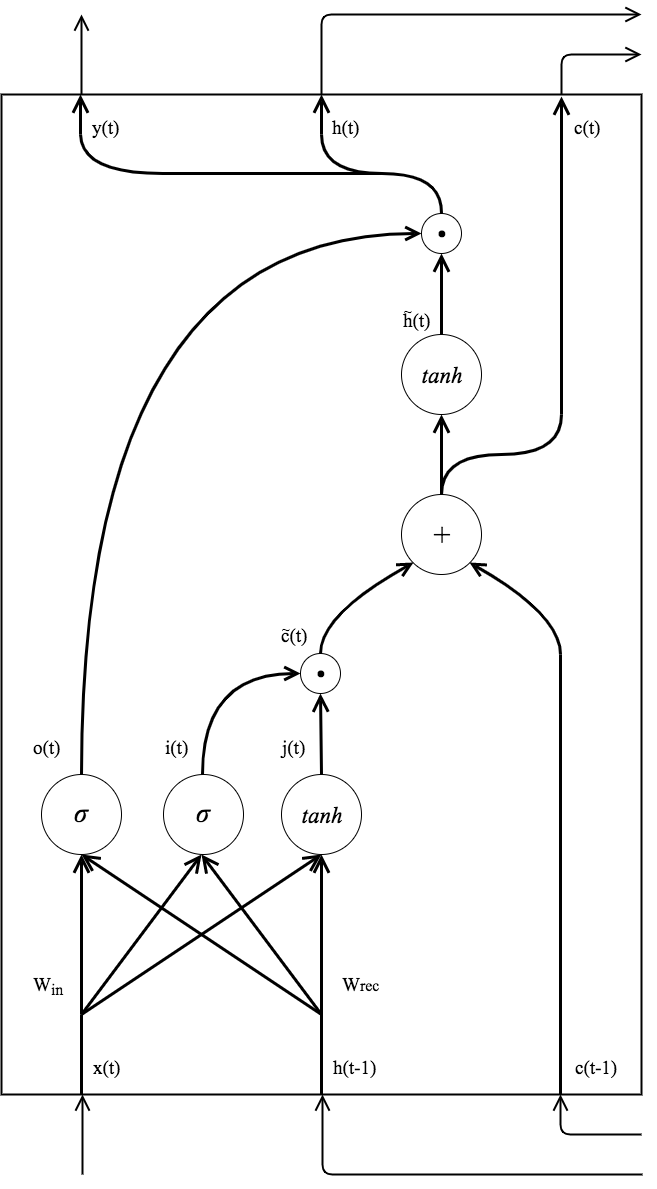
\includegraphics[scale=0.2]{formerLSTM.png}
		\caption{Flujo de información en la estructura de la celda LSTM original.}
		\label{formerLSTM}
	\end{figure}
	
	Cómo puede verse en la figura \ref{formerLSTM} la celda incorpora un vector $j(t)$ con información proveniente de las variables de entrada a partir de realizar una clasificación no lineal aplicando la función $tanh(\cdot)$ sobre el resultado de una regresión de los valores $x(t)$ de las variables de entrada y el estado $h(t-1)$ de la celda al momento de ser evaluada.\\
	La cantidad de información efectivamente incorporada dependerá de la activación de la compuerta $i(t)$. Esta compuerta realiza una regresión logística sobre los valores de las variables de entrada y el valor del estado de las celdas al momento de ser evaluada. El resultado de la regresión logística es multiplicado coordenada por coordenada con el vector $j(t)$ para obtener un nuevo vector $\tilde{c}(t)$ con información seleccionada para ser incorporada en la memoria de la celda en el instante $t$.\\
	La información seleccionada para ser incorporada a la celda y la información retenida en el estado interno $c(t-1)$ de la celda al momento de ser evaluada son sumadas para obtener el vector $c(t)$. Este vector es entonces usado como entrada a la función $tanh(\cdot)$ para obtener el vector $\tilde{h}(t)$.\\
	Finalmente la información a ser efectivamente expuesta a las capas superiores es seleccionada por la compuerta $o(t)$. Esta compuerta, análogamente a la compuerta $i(t)$ realiza una regresión logística respecto de los valores de las variables de entrada y el valor del estado de la celda al momento de ser evaluada. La selección final es obtenida de una multiplicación coordenada a coordenada de los vectores $o(t)$ y $\tilde{h}(t)$ para obtener el nuevo estado de la celda $h(t)$ en el instante $t$.\\
	
	Vale la pena destacar el funcionamiento del mecanismo de realimentación de la celda. El mismo es definido adrede para que sea una copia del estado previo de la celda. \\
	Se considera, por otro lado, que la propagación del error decae exponencialmente para las dependencias directas de las componentes $i$, $j$ y $o$ con instantes de tiempo previos debido a la sucesiva aplicación de funciones no lineales\cite{25DependenciesProblemHochreiter}.\\
	Entonces, la dependencia temporal con el estado previo es $\frac{\partial c(t+1)}{c(t)} = 1$ que, como vimos anteriormente, es el único escenario donde no se produce el problema de desvanecimiento o saturación del gradiente. La solución presentada es denominada Constant Error Carrousel(CEC).\\
	Habiendo implementado CEC, es posible obtener la señal de entrenamiento apropiada para los parámetros $\theta$ respecto a estados en instantes de tiempo muy distantes del actual según las siguientes ecuaciones
	\begin{equation}\label{temporalDependenceLSTM}
	\dfrac{\partial \mathcal{E}(t)}{\partial \theta} = \dfrac{\partial \mathcal{E}(t)}{\partial h(t)} \dfrac{\partial h(t)}{\partial \theta} =\sum_{k=0}^{t} \dfrac{\partial \mathcal{E}(t)}{\partial h(t)} \dfrac{\partial h(t)}{\partial c(t)}\dfrac{\partial c(t)}{\partial c(k)}\dfrac{\partial c(k)}{\partial \theta}
	\end{equation}
	Luego, la señal de entrenamiento es transmitida a cada instante de tiempo previo $k$ en la sumatoria a través del vector de estado interno $c(t)$ como evidencia la siguiente ecuación
	\begin{equation}\label{expandedCEC}
	\dfrac{\partial c(t)}{\partial c(k)} = \dfrac{\partial c(t)}{\partial c(t-1)} ... \dfrac{\partial c(k+1)}{\partial c(k)} = \prod_{k}^{t-1} \dfrac{\partial c(k+1)}{\partial c(k)} = 1^{t-k} = 1
	\end{equation}
	Por lo tanto, reemplazando (\ref{expandedCEC}) en (\ref{temporalDependenceLSTM}) se obtiene
	\begin{equation}\label{timeExpandedLSTM}
	\dfrac{\partial \mathcal{E}(t)}{\partial \theta} = \dfrac{\partial \mathcal{E}(t)}{\partial h(t)} \dfrac{\partial h(t)}{\partial \theta}=\sum_{k=0}^{t} \dfrac{\partial \mathcal{E}(t)}{\partial h(t)} \dfrac{\partial h(t)}{\partial c(t)}\dfrac{\partial c(k)}{\partial \theta}
	\end{equation}
	Es posible apreciar en (\ref{timeExpandedLSTM}) el que el efecto que produce el estado interno de la celda sobre el error en el instante de tiempo $t$ es análogamente considerado para instantes previos. Esta propiedad se transfiere a la señal de entrenamiento para el conjunto de parámetros $\theta$ respecto a su aporte en instantes de tiempo previos.\\
	Esta solución es indudablemente eficaz para retener dependencias temporales intactas incluso con secuencias de eventos extremadamente largas, del orden de 1000 períodos de tiempo.\\
	
	Otro aspecto destacable de las celdas LSTM lo constituyen las compuertas de selección de entrada y salida de información, $i$ y $o$ respectivamente. Las mismas son la solución propuesta a un problema sutil en las RNNs.\\
	Concretamente las compuertas mencionadas funcionan como un controlador que selecciona la información que ingresara a la celda o será expuesta como salida de la misma. Esta separación de incumbencias permite aislar la tarea de resguardar y liberar la información retenida en la celda en un componente dedicado distinto al que realiza la inferencia sobre el espacio de las variables de entrada.\\
	De esta manera la señal de error que se le atribuye a la celda es correctamente distribuida sobre los componentes dependiendo de su responsabilidad respecto del resultado expuesto.\\
	El resultado es un entrenamiento preciso de cada componente en la tarea específica que desempeñan.\\
	Comúnmente a estos componentes $i$ y $o$ se los conoce como \textit{input gate} y \textit{output gate} respectivamente.
	
	\subsection{Deriva del estado}
	A pesar de su efectividad, la formulación original de las celdas LSTM presenta problemas en aplicaciones prácticas debido a su incapacidad de resetear la información retenida en el estado interno $c(t)$ de la celda de forma autónoma. \\
	La celda requiere que se borre la información retenida al inicio de cada secuencia que no tenga relación con otros eventos previamente registrados por la celda, aun cuando la delimitación está claramente marcada en el espacio de valores de las variables de entrada.\\
	Este problema fue previsto en su publicación original bajo el nombre de deriva del estado. La manifestación del problema depende de que la tarea en la que se evalúe el modelo contenga subsecuencias sin conexión entre sí. \\
	Particularmente en el conjunto de tareas donde fue probada la estructura original ha sido suficiente con seleccionar convenientemente el valor de los sesgos $b_i$ de la compuerta de entrada $i$. Por otra parte, el estado de la celda era reseteado explícitamente al terminar cada secuencia del conjunto de tareas donde la estructura de la celda LSTM fue probada originalmente\\
	Luego de la publicación de la estructura original de la celda LSTM se propuso una modificación que contempla específicamente el problema de deriva del estado\cite{16ForgateGatePeepholeConnectionsGers}. La nueva formulación de la celda LSTM introduce una nueva compuerta $f$ encargada de borrar la información almacenada en el estado de la celda en función de las entradas y de el estado previo del la misma.\\
	
	La modificación propuesta como solución al problema de la deriva del estado afecta únicamente al cálculo del estado interno de la celda según las ecuaciones
	\begin{equation*}
	f(t) = f_2(W_{in, f} x(t) + W_{rec, f} h(t-1) + b_f)
	\end{equation*}
	\begin{equation*}
	c(t) = f(t)c(t-1) + i(t)j(t)
	\end{equation*}
	donde la compuerta $f$ constituye un modulo análogo a las compuertas $i$ e $o$ que actúa sobre la realimentación del estado interno previo de la celda, seleccionando bajo una condición de sus variables de entrada la proporción del estado previo que se preservara en el instante actual. Esta nueva compuerta $f$ es denominada \textit{forget gate}.\\
	
	La figura \ref{vanillaLSTM} muestra la estructura de la celda LSTM con la modificación diseñada para solucionar el problema de la deriva del estado.
	\begin{figure}[H]
		\centering
		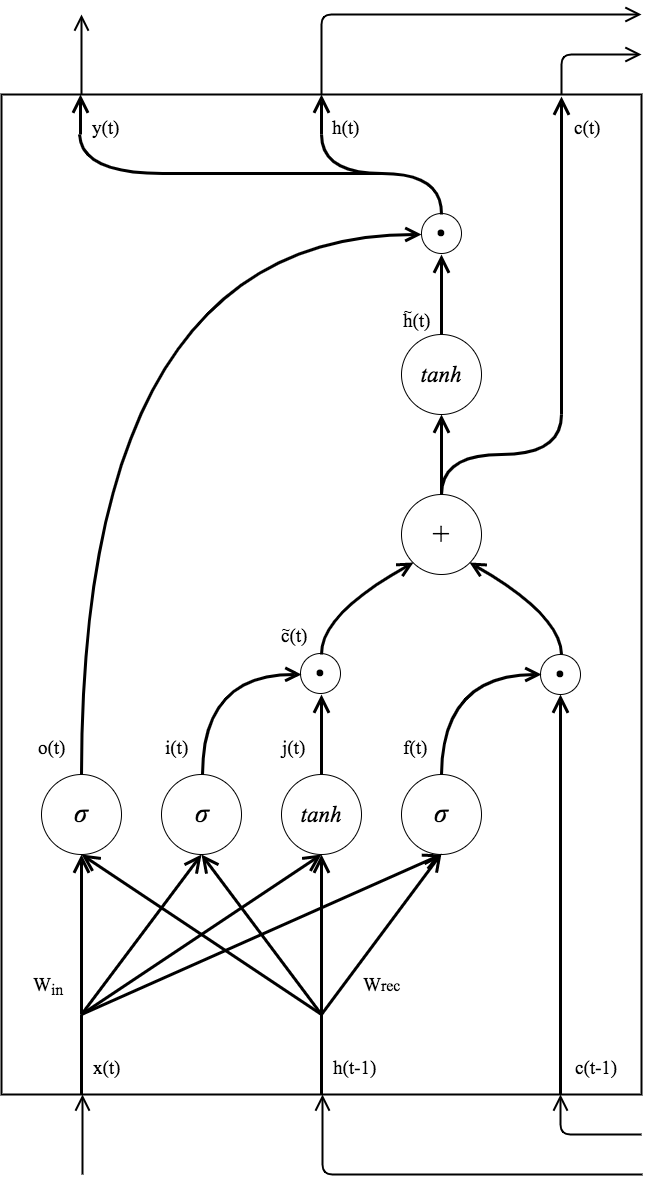
\includegraphics[scale=0.2]{vanillaLSTM.png}
		\caption{Estructura de la celda LSTM modificada para incluir la compuerta $f$.}
		\label{vanillaLSTM}
	\end{figure}
	
	Puede verse en la figura \ref{vanillaLSTM} que la cantidad de información a retener proveniente de previas evaluaciones de la celda y presente en el valor del vector $c(t-1)$ es seleccionada para evitar el problema de la deriva del estado. La compuerta $f(t)$ realiza una regresión logística respecto de los valores de las variables de entrada $x(t)$ y el valor del estado $h(t-1)$ de la celda al momento de ser evaluada, de forma análoga a las compuertas $i$ y $o$ ya descritas. Por lo tanto, la selección se realiza con una multiplicación coordenada por coordenada de los vectores $f(t)$ y $c(t-1)$.\\
	
	Es oportuno destacar el efecto que tiene esta modificación sobre el ya expuesto problema del gradiente debido a que la nueva formulación del cálculo del estado introduce la multiplicación del estado interno de la celda $c(t)$ con el valor de la compuerta $f(t)$, cuya imagen cumple $f(t) \in (0, 1)$.\\
	Implementando la compuerta $f$ la dependencia truncada del estado interno de la celda en el instante $t$ con el instante de tiempo inmediatamente anterior esta dada por
	\begin{equation}\label{forgetGateDependency}
	\dfrac{\partial c(k+1)}{\partial c(k)} = \dfrac{\partial (c(k) \, f(k+1))}{\partial c(k)} = f(k+1) + \underbrace{\dfrac{\partial f(k+1)}{\partial c(k)}}_{\rightarrow 0}
	\end{equation}
	Por lo tanto, reemplazando (\ref{forgetGateDependency}) en la formulación de la dependencia entre instantes de tiempo $t$ y $k$, tal que $k \le t$, se obtiene
	\begin{equation}\label{forgetGateCEC}
	\dfrac{\partial c(t)}{\partial c(k)} = \dfrac{\partial c(t)}{\partial c(t-1)} ... \dfrac{\partial c(k+1)}{\partial c(k)} = \prod_{k}^{t-1} \dfrac{\partial c(k+1)}{\partial c(k)} = \prod_{k}^{t-1} f(k+1)
	\end{equation}
	Como puede apreciarse en (\ref{forgetGateCEC}), a diferencia de la implementación original de la celda LSTM, la modificación que incluye la compuerta $f$ introduce un factor que le permite a la celda borrar tanto el registro de la información contenida como la propagación de errores hacia instantes de tiempo previos, ``olvidando" los errores cometidos.\\
	Otro aspecto destacable es que dado que $f$, cumple que $f(t) \in (0, 1)$, entonces la dependencia con un estado interno previo debería tender a desvanecerse para secuencias de eventos muy largas ya que $x^l \xrightarrow[l \to \infty]{} 0, \forall x \in (0,1)$. \\
	Comúnmente, y particularmente al inicio del entrenamiento, este problema es abordado seleccionando el sesgo $b_f$ para que provea valores de $f(t)$ cercanos a 1. A pesar de este problema el desempeño de las celdas LSTM sobre experimentos con amplias secuencias de eventos no decae exponencialmente con el crecimiento de la longitud de la secuencia.\\
	Esta observación indica que posiblemente la celda es capaz de compensar la pérdida de información aumentando ligeramente el estado interno $c$ en forma constante a través de la actualización no recurrente del mismo dada por la adición el vector $\tilde{c}(t) = i(t)j(t)$.
	
	\subsection{Conteo preciso}
	Un tipo de tarea en particular presenta un desafío para las RNNs y por consiguiente a las celdas LSTM, este problema es el conteo preciso de tiempo.\\
	En este tipo de tareas se tiene una señal periódica que no provee mayor información que un cambio abrupto separado por intervalos de tiempo fijo. Un ejemplo simple de estas señales lo constituyen picos de actividad separados por intervalos de tiempo fijos e iguales.\\
	Sobre este escenario la única información disponible para la celda LSTM es una entrada constante de tiempo durante la mayor parte del periodo y se espera que prediga con exactitud el instante en el que se producirá el cambio abrupto en forma periódica. Luego, la celda deberá valerse de su estado interno para almacenar la cantidad de tiempo transcurrido y predecir con exactitud la manifestación del pico de la señal.\\
	
	La estructura de la celda LSTM incluyendo la compuerta $f$, definida en la sección anterior presenta problemas al momento de exponer predecir con exactitud la periodicidad de la señal debido a la secuencia de operaciones realizadas para exponer una salida.\\
	Particularmente al presentar un valor de las variables de entrada los distintos componentes de la celda toman esa información en conjunto con el estado previo de la celda para inferir una salida, seguidamente se opera entre estas salidas parciales de cada componente para obtener el resultado expuesto.\\
	Según el proceso descrito cada uno de los componentes desconoce el valor de los otros y más aún, desconocen el estado interno de la celda al realizar su inferencia y exponer un resultado parcial. Esto es de particular importancia en la compuerta de salida ya que la misma no tiene la información precisa del estado que está exponiendo.\\
	Este detalle es de crucial importancia en la tarea descrita ya que un retraso de un instante de tiempo en la exposición de la salida adecuada implica un error muy grande en el resultado.\\
	
	Para solucionar este problema y enriquecer a las celdas LSTM con un mecanismo que le permita realizar conteos precisos se propuso una nueva modificación en su estructura, esta vez añadiendo conexiones internas entre el estado interno de la celda y cada uno de los componentes que participan en el cálculo de la salida expuesta.\\
	Entonces formalmente la celda LSTM con conexiones internas queda definida por las siguientes ecuaciones en el orden dado
	\begin{equation*}
	\begin{split}
	j(t) &= f_1(W_{in, j} x(t) + W_{rec, j} h(t-1) + W_{pep, j} c(t-1) + b_{j})\\
	i(t) &= f_2(W_{in, i} x(t) + W_{rec, i} h(t-1) + W_{pep, i} c(t-1) + b_{i})\\
	f(t) &= f_2(W_{in, f} x(t) + W_{rec, f} h(t-1) + W_{pep, f} c(t-1) + b_f)\\
	c(t) &= f(t)c(t-1) + i(t)j(t)\\
	o(t) &= f_2(W_{in, o} x(t) + W_{rec, o} h(t-1) + W_{pep, o} c(t) + b_o)\\
	h(t) &= o(t)f_1(c(t))\\
	y(t) &= h(t)
	\end{split}
	\end{equation*}
	donde las matrices $W_{pep}$ ponderan los valores del estado interno actual al momento de realizar la inferencia en cada componente.\\
	Nótese que en el caso de la compuerta $o$ la ponderación se realiza con el estado interno recientemente calculado en vez que con el obtenido en el instante $t-1$ anterior.	Estas conexiones internas fueron denominadas \textit{peephole connections}.
	
	\subsection{Regularización}
	Una mejora aun no explorada es la regularización de la RNN por el método Dropout. Este método es ampliamente usado en redes neuronales en general y constituye una herramienta muy valiosa en redes neuronales con una gran cantidad de parámetros.\\
	El método de regularización Dropout busca reducir el overfitting en redes neuronales a partir de descartar las salidas de las celdas de forma aleatoria con una probabilidad $p$. Esta probabilidad es un parámetro a seleccionar por el usuario.\\
	
	El racional detrás de este método de regularización radica en que descartando la salida de las celdas de forma aleatoria se evita que los componentes en capas superiores conectados con la salida de estas desarrollen una fuerte dependencia con los valores de los parámetros que los conectan.\\
	Básicamente el mecanismo de regulación Dropout puede considerarse como la adición de ruido inducido sobre la red neuronal. Seguidamente se exige a la red neuronal que omita el ruido presentado, desarrollando así una representación interna que exitosamente extraiga las conexiones relevantes en la red.\\
	
	En la práctica el método de regularización provee una apreciable mejora del desempeño reduciendo el error en la generalización, discutido en la sección \ref{sectionRNN}.\\
	Es oportuno mencionar que la regularización por Dropout puede aplicarse tanto sobre las salida de las celdas LSTM como a sobre las variables de entrada. Análogamente este mecanismo puede usarse en otras NNs, especialmente en otras RNNs.\\
	
	Otro tipo de métodos de regularización de parámetros también pueden ser aplicados independientemente de la aplicación del método Dropout. Estos métodos forman parte del estudio del problema de generalización en NNs que, como se mencionó anteriormente, es un tema de estudio muy amplio que no será explorado en mayor detalle en la presente investigación.
	
	\subsection{Aprendizaje residual}
	La difusión de los modelos que apilan una amplia cantidad de capas de neuronas en una única red neuronal desbloqueó niveles de desempeño nunca antes obtenidos en el campo de machine learning. Particularmente el campo de visión computarizada fue receptor de múltiples arquitecturas novedosas que establecieron un nuevo estándar de desempeño, más allá del obtenido por los humanos\cite{27DNNAgainstHumans}. No obstante la agregación de múltiples capas de neuronas se ha convertido en un patrón frecuente en NNs en general debido a las mejoras en desempeño obtenidas por la explotación de una mayor capacidad de la red para tener representaciones internas de los datos de entrada.\\
	
	Sin embargo, incorporar incrementalmente capas de redes neuronales significó la manifestación de problemas incrementalmente más complejos en el entrenamiento de la red resultante\cite{6Generalization}.\\
	Este hecho fue explorado en profundidad concluyéndose que no se debía al ya mencionado problema de overfitting. En cambio, los experimentos realizados sobre estas redes\cite{28ResidualLearning} con un amplio número de capas, del orden de 10 hasta 1000 capas, mostraron que se produce una saturación en el desempeño de la red donde no se obtienen ventajas en el desempeño por la inclusión de más capas, y luego del cual el desempeño empeora drásticamente si se siguen agregando capas.\\
	
	Considerando la aún no resuelta relación entre los modelos de una reducida cantidad de capas respecto de su contraparte con una amplia cantidad de capas, se contempló el caso ya mencionado donde un modelo que se encuentra en la zona de saturación de desempeño y el caso de una versión aumentada en capas del mismo, cuyo desempeño es peor al original. Teóricamente debería ser posible para el modelo con mas capas igualar el desempeño del modelo original a partir de configurar los parámetros de las capas adicionales para que igualen la matriz identidad y de esta manera resuelvan la copia del resultado del modelo original. En la práctica se encuentra que esta configuración mencionada en la que se copia la salida resuelta por una capa inferior no es fácilmente obtenida de la optimización del conjunto de parámetros $\theta$\cite{28ResidualLearning}.\\
	
	Se propuso entonces un esquema distinto donde se facilita esta copia de las salidas de las capas previas para resolver la perdida del desempeño observada y de esta forma explotar la capacidad aumentada de las NNs con un mayor cantidad de capas.\\
	Concretamente, si se considera la salida prevista por un conjunto de capas de una red como un mapeo $\mathcal{H}$ de las entradas $x$, entonces se optimizan los parámetros $\theta^l, ... , \theta^{l+n}$ de las capas $l, ... , l+n$ de forma tal que representen el nuevo mapeo residual $\mathcal{F}$ de las entradas $x$, tal que $\mathcal{F}(x) = \mathcal{H}(x) - x$. Finalmente se adiciona de forma explícita las entradas $x$, siendo el resultado de la evaluación de la capa igual a $\mathcal{F}(x) + x$.\\
	Optimizar los parámetros $\theta^l, ... , \theta^{l+n}$ de las capas $l, ... , l+n$ para que aproximen el mapeo residual $\mathcal{F}$ cuando $\mathcal{H} = \mathbb{I}$ es una tarea más sencilla debido a que en este caso es suficiente con configurar los parámetros para que sean igual a $0$ en todos los casos y simplemente se copien las entradas $x$\cite{28ResidualLearning}.\\
	La conveniencia de este esquema radica en que se referencia la salida de las $n+l$ capas respecto de la entrada de la primer capa $l$, pudiendo obtenerse más fácilmente una aproximación a la función identidad que en el caso de apilar múltiples capas no lineales sin referencia a las entradas para aproximar la función identidad.\\
	
	El esquema de aprendizaje residual es obtenible a partir del uso conveniente de un patrón de arquitectura de NNs denominado \textit{shortcut connections}\cite{29ShortcutConnections} donde se conectan en forma ponderada las salidas de capas inferiores con las capas superiores, más cercanas a la resolución de la salida de la red. En el caso del aprendizaje residual la ponderación se realiza especificando que la matriz de pesos que referencia la salida de la capa $l+n$ respecto de la salida de la capa $l-1$ sea igual a la identidad.\\
	
	En el caso de las RNNs el esquema de aprendizaje residual pueden emplearse análogamente a su aplicación en las NNs para referenciar las salidas de capas superiores, más cercanas a la salida, con la salida de capas inferiores.\\
	Particularmente será útil la aplicación de este esquema al momento de implementar la modificación sobre la estructura original de las celdas LSTM en la sección siguiente, debido a que dicha modificación aplica en forma iterativa un mapeo sobre las entradas originales luego del cual es conveniente referenciar las salidas de las celdas con las entradas de las mismas. Esta propiedad constituye un primer indicio de la relación que existe entre realizar múltiples iteraciones sobre la evaluación de una capa de celdas LSTM y la agregación de múltiples capas sin pesos compartidos.
	
	\pagebreak
	\section{LSTM iterativa}\label{sectionIterativeLSTM}
	En esta sección se detalla la modificación en la estructura de las celdas LSTM propuesta como resultado del estudio de las RNNs desde la perspectiva de los sistemas dinámicos.\\
	Según lo expuesto en la sección \ref{sectionRNN} las RNNs mencionadas describen sistemas dinámicos no homogéneos donde el estado interno de las celdas evoluciona con cada evaluación de la misma.\\
	Adicionalmente, dependiendo del valor del conjunto de parámetros $\theta$, la dinámica descrita por la formulación de la RNN y el estado inicial de la red, la evolución del estado de la celda puede verse inmersa en la cuenca de un punto fijo denominado atractor. Bajo estas condiciones y mientras no se registre la presencia de nueva información relevante que lleve el estado fuera de la cuenca del atractor, la evolución del estado en sucesivas evaluaciones se mantendrá dentro dicho dominio, reteniendo de esa forma la información registrada por la celda. En este caso la representación de la información retenida es expuesta en la forma de los estados pertenecientes a la cuenca del atractor asociado a la respectiva información.\\
	
	Sin embargo, representar la información retenida en forma de un dominio de estados posibles implica que en las fronteras de estos dominios pueden darse clasificaciones erróneas por los componentes que interpreten la salida de las RNNs para inferir y exponer una salida, con la intención de predecir el valor de una variable aleatoria.\\
	Estas clasificaciones dependen de la correcta alineación de los hiperplanos correspondientes a los componentes que interpreten la salida de la RNN con las fronteras de las cuencas de los atractores. Por lo tanto, las fronteras difusas	donde se mezclen los estados pertenecientes a los distintos dominios o las fronteras delimitadas por superficies irregulares aumentarán el error en la clasificación de los patrones presentes en el dominio de las variables de entrada propios de la tarea de clasificación de la red.\\
	
	Explotando las propiedades de evolución de los sistemas dinámicos se propone la realización de sucesivas evaluaciones de la celda sobre los mismos valores de entrada, con la intención de guiar el estado interno de la celda hacia un dominio dentro de la cuenca del atractor más reducido que el resultante de una única evaluación de la celda. Este dominio tiene una menor superficie y agrupa los estados que representan la información retenida en posiciones más próximas al atractor correspondiente.\\
	Luego, la condición de convergencia descrita aplica a todos los estados posibles de la celda guiándolos al atractor correspondiente a la cuenca de atracción en la que se ubica el estado de la celda al momento de realizar la inferencia. \\
	Como será expuesto más adelante, las trayectorias que describan los sucesivos estados de la celda en su evolución no pueden intersecarse en ningún punto, por lo tanto las superficies que delimiten las cuencas de atracción se separaran y/o simplificarán con cada iteración realizada, permitiendo una clasificación mas precisa por los hiperplanos de los componentes que interpreten la salida de la RNN para predecir el valor de una variable aleatoria.\\
	Formalmente, se define la dinámica del estado interno de la red descrita por la celda LSTM es
	\begin{equation*}
	\begin{split}
	j(t) &= f_1(W_{in, j} x(t) + W_{rec, j} h(t-1) + b_{j})\\
	i(t) &= f_2(W_{in, i} x(t) + W_{rec, i} h(t-1) + b_{i})\\
	f(t) &= f_2(W_{in, f} x(t) + W_{rec, f} h(t-1) + b_f)\\
	c(t) &= f(t)c(t-1) + i(t)j(t)\\
	o(t) &= f_2(W_{in, o} x(t) + W_{rec, o} h(t-1) + b_o)\\
	h(t) &= o(t)f_1(c(t))
	\end{split}
	\end{equation*}
	\begin{equation}\label{LSTMdynamics}
	\dfrac{\partial h(t-1)}{\partial t} = h(t) - h(t-1) = f(h(t-1), x(t))
	\end{equation}
	donde la formulación dada corresponde a una celda LSTM que no incorpora la mejora descrita en la sección \ref{sectionIterativeLSTM} para el conteo preciso debido a que no es un requerimiento propio de las tareas a evaluar. Según (\ref{LSTMdynamics}), la formulación de la celda LSTM empleada describe un sistema dinámico no homogéneo el cual ya se anticipó en la sección \ref{sectionRNN} que es una característica de las RNNs en general.\\
	Luego, considerando la modificación mencionada los valores de las variables de entrada $x(t)$ permanecen constantes por lo tanto la evolución del estado $h(t)$ del sistema durante sucesivas evaluaciones de la celda está completamente determinada por el valor de las condiciones iniciales $x(t)$, $c(t-1)$ y $h(t-1)$. Formalizando estas condiciones y agrupando los términos constantes se obtiene la siguiente formulación del sistema dinámico durante sucesivas iteraciones
	
	\begin{equation*}
	\begin{split}
	j(\tau) &= f_1(W_{rec, j} h + \underbrace{W_{in, j} x(t) + b_{j}}_{C_j} ) =  f_1(W_{rec, j} h + C_j)\\
	i(\tau) &= f_2(W_{rec, i} h + \underbrace{W_{in, j} x(t) + b_{j}}_{C_i} ) =  f_1(W_{rec, i} h + C_i)\\
	f(\tau) &= f_2(W_{rec, f} h + \underbrace{W_{in, j} x(t) + b_{j}}_{C_f} ) =  f_1(W_{rec, f} h + C_f)\\
	c(\tau) &= f(\tau)\underbrace{c(t-1)}_{c_0} + i(\tau)j(\tau) = f(\tau) c_0 + i(\tau)j(\tau) \\
	o(\tau)& = f_2(W_{rec, o} h + \underbrace{W_{in, j} x(t) + b_{j}}_{C_o} ) =  f_1(W_{rec, o} h + C_o)\\
	h(\tau) &= o(\tau)f_1(c(\tau))
	\end{split}
	\end{equation*}
	\begin{equation}\label{iterativeLSTMdynamics}
	\dfrac{\partial h}{\partial \tau} = h(\tau) - h = f(h(\tau))
	\end{equation}
	donde se analiza la dinámica sobre la escala de tiempo $\tau$ que distingue entre sucesivas iteraciones y que es menor que la escala de tiempo $t$ que distingue entre sucesivos entre instantes de la secuencia de entrada. Los términos $C_j, C_i, C_f, C_o$ son constantes en la escala de tiempo $\tau$ ya que dependen del valor de las variables de entrada $x(t)$. La constante $c_0$ es el valor del estado interno de la celda en el instante $t-1$, antes de comenzar a realizar sucesivas evaluaciones. \\
	Este sistema, análogamente al descrito por las RNNs en general, es un mapa\cite{21StrogatzBook}.\\
	Es oportuno destacar que la celda LSTM iterativa no modifica el estado interno de la celda hasta el momento de emitir un resultado, de esta forma las dependencias temporales pueden ser preservadas evitando el problema de desvanecimiento del gradiente como se expondrá más adelante en esta sección.
	
	\subsection{Evolución del sistema entre iteraciones}
	Realizando un análisis similar al expuesto en la sección \ref{sectionRNN}, se estudiará la dinámica de la celda LSTM iterativa definida en (\ref{iterativeLSTMdynamics}).\\
	Considerando la linealización del sistema obtenida por la expansión en series de Taylor de la función $f$ y considerando el cambio de variables $v(\tau) = (h(\tau) - h^*)$ en un entorno de un punto fijo $h^*$ se obtiene
	\begin{equation*}
	\dfrac{\partial h(\tau)}{\partial \tau} = f(h) = f(h^*) + \dfrac{\partial f(h^*)}{\partial h_1} \, v_1+ ... + \dfrac{\partial f(h^*)}{\partial h_n} \, v_n + O(v_1^2, v_1 \, v_2, ... , v_n^2)
	\end{equation*}
	\begin{equation*}
	\dfrac{\partial h(\tau)}{\partial \tau} = \dfrac{\partial v(\tau)}{\partial \tau} = f(h^*) + \mathrm{J}_f(h^*) \, v + O(v \, v^T)
	\end{equation*}
	donde $v_i$ son las coordenadas del vector $v(\tau)$ en cada iteración de la escala de tiempo $\tau$. $h^*$ son las coordenadas del punto fijo en el instante $t$, y por consiguiente en todas las iteraciones. $\mathrm{J}_f(h^*)$ es el jacobiano de $f$ evaluado en el punto fijo $h^*$. \\
	Para simplificar notación no se explicitó la dependencia del punto fijo $h^*$ respecto de la escala de tiempo $t$, pero el lector debe recordar que la ubicación del punto fijo está determinada por la formulación de la dinámica de la celda y el conjunto de parámetros que forman parte de dicha formulación, en este caso son las matrices  $W_{rec, j}, W_{rec, i}, W_{rec, f}, W_{rec, o}$ y los vectores $C_j, C_i, C_f, C_o$. Estos últimos dependen del instante de tiempo $t$ en forma directa a través de los valores de las variables de entrada.\\
	
	Luego, considerando que $f(h^*) = 0$ y teniendo en cuenta que dentro de un entorno cercano al punto fijo $h^*$ se discrimina el efecto de los términos de mayor orden a los lineales se obtiene la aproximación
	\begin{equation}\label{linearDynamics}
	\begin{split}
	\dfrac{\partial h(\tau)}{\partial \tau} &= \mathrm{J}_f(h^*) \, (h(\tau) - h^*)\\
	\dfrac{\partial v(\tau)}{\partial \tau} &= \mathrm{J}_f(h^*) \,v(\tau) 
	\end{split}
	\end{equation}
	
	Contemplando que el próximo estado del sistema esta determinado en función del estado actual y la variación instantánea del estado según la ya explorada ecuación (\ref{iterativeLSTMdynamics}) se tiene
	\begin{equation}\label{recurrentStateCalculation}
	h(\tau) = \dfrac{\partial h(\tau -1)}{\partial \tau} + h(\tau -1)
	\end{equation}
	análogamente puede definirse la evolución del $v(\tau)$ como 
	\begin{equation}\label{recurrentVCalculation}
	v(\tau) = \dfrac{\partial v(\tau -1)}{\partial \tau} + v(\tau -1)
	\end{equation}
	entonces es posible obtener la secuencia de estados intermedios producto de la realización $n$ iteraciones a partir de aplicar de forma recurrente la ecuación (\ref{recurrentVCalculation}) reemplazando apropiadamente la variación instantánea descrita en (\ref{linearDynamics})
	\begin{equation}\label{preInductionStep}
	v(\tau) = \dfrac{\partial v(\tau -1)}{\partial \tau} + v(\tau -1) = \mathrm{J}_f(h^*) \, v(\tau -1) + v(\tau -1) = (\mathrm{J}_f(h^*) + \mathbb{I}) \, v(\tau -1)
	\end{equation}
	donde $\mathbb{I}$ es la matriz identidad. Luego, por inducción sobre (\ref{preInductionStep}) se obtiene la siguiente relación entre el estado al iniciar las $n$ iteraciones y el estado final
	\begin{equation*}
	v(\tau) = (\mathrm{J}_f(h^*) + \mathbb{I}) v = (\mathrm{J}_f(h^*) + \mathbb{I}) \, (\mathrm{J}_f(h^*) + \mathbb{I})  \, v(\tau-2)
	\end{equation*}
	\begin{equation*}
	v(\tau) = (\mathrm{J}_f(h^*) + \mathbb{I})^n \, v(\tau-n) = (\mathrm{J}_f(h^*) + \mathbb{I})^n \, v(t-1)
	\end{equation*}
	Entonces, es posible obtener las condiciones que debe cumplir el sistema para que iterativamente los estados dentro de la cuenca del atractor converjan al punto fijo $h^*$, pidiendo que $||v(\tau)||\xrightarrow[\tau \to \infty]{} 0$
	\begin{equation*}
	||v(\tau)|| \xrightarrow[\tau \to \infty]{} 0 \iff ||(\mathrm{J}_f(h^*) + \mathbb{I})^\tau \, v(t-1)|| \xrightarrow[\tau \to \infty]{} 0
	\end{equation*}
	Por otra parte, considerando la base de autovectores ${ u_1, \,... \,, u_n }$ de la matriz $\mathrm{J}_f(h^*)$ asociados a los autovalores $\lambda_1, ... , \lambda_n$, es posible escribir el vector $v$ en términos dicha base como $v(t) = \sum_{i=1}^{n} c_i u_i$. Entonces se obtiene
	\begin{equation*}
	||v(\tau)|| = ||(\mathrm{J}_f(h^*) + \mathbb{I})^\tau \, \sum_{i=1}^{n} c_i u_i|| = || \sum_{i=1}^{n} c_i  (\mathrm{J}_f(h^*) + \mathbb{I})^\tau \, u_i||
	\end{equation*}
	Aplicando el teorema que relaciona los autovalores y autovectores de una matriz $A$ y una matriz $p(A)$, siendo $p(x)$ un polinomio de grado $k$, se tiene que los autovalores de $p(A)$ serán $p(\lambda_1), \,... \,, p(\lambda_n)$ donde $\lambda_1, \,... \,, \lambda_n$ son los autovalores de $A$ con su multiplicidad. \\
	Entonces, considerando primero el polinomio de grado 1, $p_1(x) = x + \mathbb{I}$, los autovalores de $p_1(\mathrm{J}_f(h^*)) = \mathrm{J}_f(h^*) + \mathbb{I}$ serán $\lambda_1 + 1, ... \,, \lambda_n + 1$ respectivamente, siendo $\lambda_1, \,... \,, \lambda_n$ son los autovalores de $\mathrm{J}_f(h^*)$. \\
	Luego considerando el polinomio de grado $\tau$, los autovalores de $p_2(p_1(x)) = (\mathrm{J}_f(h^*) + \mathbb{I})^\tau$ serán $(\lambda_1 + 1)^\tau, \,... \,, (\lambda_n + 1)^\tau$, nuevamente siendo $\lambda_1, \,... \,, \lambda_n$ son los autovalores de $\mathrm{J}_f(h^*)$.\\
	
	Resumiendo el cálculo de las condiciones para la convergencia de los estados en la cuenca del atractor hacia el punto fijo $h^*$, según lo visto es posible obtener condiciones para los autovalores $\lambda_1, \,... \,, \lambda_n$ de $\mathrm{J}_f(h^*)$, relacionando los mismos con la norma del vector $v(\tau)$ y aprovechando su descomposición en la base de autovectores ${ u_1, \,... \,, u_n }$ de la matriz $\mathrm{J}_f(h^*)$
	\begin{equation*}
	||v(\tau)||  = || \sum_{i=1}^{n} c_i  (\mathrm{J}_f(h^*) + \mathbb{I})^\tau u_i|| = || \sum_{i=1}^{n} c_i  (\lambda_i + 1)^\tau u_i||
	\end{equation*}
	Entonces, planteando las condiciones para la convergencia de $v(\tau)$ hacia el origen
	\begin{equation*}
	||v(\tau)|| \xrightarrow[\tau \to \infty]{} 0 \iff || \sum_{i=1}^{n} c_i  (\lambda_i + 1)^\tau u_i|| \xrightarrow[\tau \to \infty]{} 0
	\end{equation*}
	Sin embargo, considerando un vector $v(\tau)$ genérico se tiene que sus coordenadas $c_1, ... , c_n$ en la base de autovectores ${ u_1, ... , u_n }$ de la matriz $\mathrm{J}_f(h^*)$ cumplen $c_i \neq 0, i = 1, ..., n$ ya que de otra forma se tendría el caso trivial $v(\tau) = 0$. Por lo tanto se obtiene
	\begin{equation*}
	\begin{split}
	||(h(\tau) - h^*)|| = ||v(\tau)|| \xrightarrow[\tau \to \infty]{} 0 &\iff |(\lambda_i + 1)^\tau| \xrightarrow[\tau \to \infty]{} 0 \quad i = 1, ..., n\\
	&\iff |\lambda_i + 1| < 1 \quad i = 1, ..., n
	\end{split}
	\end{equation*}
	Este resultado implica que para satisfacer la condición de convergencia hacia el punto fijo los autovalores de $\mathrm{J}_f(h^*)$ deben pertenecer al circulo abierto de números complejos centrado en $-1$.\\
	Cumpliéndose las condiciones encontradas para la convergencia resulta que
	\begin{equation*}
	h(\tau) \xrightarrow[\tau \to \infty]{} h^* \iff |\lambda_i + 1| < 1 \quad i = 1, ..., n
	\end{equation*}
	para un estado inicial $h(\tau = 0) = h(t-1)$ perteneciente a un entorno del punto fijo $h^*$. \\
	Esta hipótesis de cercanía con el punto fijo atractor es una limitante necesaria para realizar un análisis lineal del sistema y su validez dependerá de el aporte de los términos no lineales a la variación instantánea del estado.\\
	Recientemente, en Laurent et.al(2016)\cite{11Laurent} se expone el comportamiento caótico del sistema en condiciones específicas. Particularmente, dicha publicación analiza el comportamiento frente a valores constantemente nulos de las variables de entrada al realizar 200 iteraciones.\\
	A pesar de que estas condiciones difieren ampliamente respecto de las propuestas, el carácter caótico del sistema para un gran número de iteraciones sugiere que mucha información del sistema es aportada por términos no lineales ya que estos son los únicos capaces de producir dicho comportamiento\cite{21StrogatzBook}.\\
	
	Para proveer un análisis más riguroso del sistema no lineal modelado y extraer condiciones que contemplen el aporte de los términos no lineales a la variación del estado se calcularán las condiciones necesarias para lograr la convergencia hacia el punto fijo $h^*$ evitando el comportamiento caótico descrito.\\
	Concretamente se expondrá la sensibilidad del resultado del sistema al variar las condiciones iniciales $h_0$ en una cantidad $\delta_0$ infinitesimalmente chica.\\
	Formalmente se describe la variación respecto del resultado final del sistema al finalizar $n$ iteraciones como 
	\begin{equation*}
	|\delta_n| = |\delta_0| e ^{n\lambda} 
	\end{equation*}
	\begin{equation*}
	\dfrac{|\delta_n|}{|\delta_0|} =  e ^{n\lambda} 
	\end{equation*}
	\begin{equation*}
	\lambda = \dfrac{1}{n} \ln\left\lvert\dfrac{\delta_n}{\delta_0}\right\rvert
	\end{equation*}
	donde $\delta_n$ es la variación respecto del resultado de realizar $n$ iteraciones. $\lambda$ es un vector tal que cada una de sus coordenadas $\lambda_i$ es conocido como el exponente Liapunov y el valor que toma define el comportamiento del sistema en la $i$-ésima dimensión, siendo caótico para $\lambda > 0$ y convergente para $\lambda < 0$\cite{21StrogatzBook}.\\
	
	Contemplando la importancia de los coeficientes de Liapunov para obtener el comportamiento convergente deseado se desarrolló en forma teórica la dependencia de los mismos respecto del conjunto de parámetros de modelo recurrente estudiado obteniendo el teorema \ref{iterativeLSTMConvergenceTheorem}. Este resultado constituye el elemento teórico más importante para justificar la mejora propuesta.
	
	\begin{theorem}
		\label{iterativeLSTMConvergenceTheorem}
		Sea $f(x(t), h(t-1), c(t-1))$ un modelo constituido por un bloque de celdas LSTM tal que
		\begin{equation*}
		h(t) = f(x(t), h(t-1), c(t-1)) =  LSTM(x(t), h(t-1), c(t-1))
		\end{equation*}
		donde $x(t)$ es el valor de las variables de entrada en el instante $t$, $c(t-1)$ y $h(t-1)$ son vectores con el valor del estado interno y del estado expuesto del bloque de celdas al momento de ser evaluado, respectivamente.\\
		Sea el sistema dinámico definido por las sucesivas evaluaciones de $f$ realizadas en $\tau$ iteraciones tal que
		\begin{equation*}
		\dfrac{\partial h}{\partial \tau} = h(\tau) -  h(\tau-1) = f(x(t), h(\tau-1), c(t-1)) - h(\tau-1) = g(h(\tau-1)) - h(\tau-1)
		\end{equation*}
		donde $g(h(\tau-1))$ constituye una función análoga a la aplicación del modelo $f(x(t), h(t-1), c(t-1))$ donde los valores de $x(t)$ y $c(t-1)$ se consideran constantes.
		Bajo estas condiciones se encuentra que
		\begin{equation*}
		\sigma_j + \frac{1}{4} \sigma_i + \frac{1}{4} \sigma_f + \frac{1}{4} \sigma_o < 1 \implies \lambda < 0
		\end{equation*}
		donde $\sigma_j$, $\sigma_i$, $\sigma_f$ y $\sigma_o$ son los valores singulares principales de las matrices que ponderan las conexiones recurrentes en las compuertas $j$, $i$, $f$ y $o$ del bloque de celdas LSTM respectivamente, y $\lambda$ es un vector tal que sus coordenadas $\lambda_i$ son los exponentes Liapunov del sistema dinámico en la $i$-ésima dimensión.
	\end{theorem}
	\begin{proof}
		Véase Apéndice \ref{iterativeLSTMconvergence}.
	\end{proof}
	
	La implicancia principal del teorema \ref{iterativeLSTMConvergenceTheorem} es que existen valores para los parámetros de las matrices $W_{rec,j}$, $W_{rec,i}$, $W_{rec,f}$ y $W_{rec,o}$ que producen el comportamiento convergente deseado. Por lo tanto los parámetros del modelo pueden ser optimizados para que el estado que es expuesto por el bloque de celdas LSTM converja iterativamente hacia el atractor de la cuenca donde se encuentra el mismo al momento de realizar la inferencia.\\
	
	Tomando los cálculos del Apéndice \ref{iterativeLSTMconvergence} donde se encuentra que para un vector de estado $h$ genérico $\left\lvert \frac{\partial g(h)}{\partial h} \right\rvert < 1$ y considerando que en un entorno cercano al punto fijo es posible realizar la aproximación lineal $\frac{\partial g(h)}{\partial h} = \mathrm{J}_f(h^*) + \mathbb{I}$, entonces se deduce la siguiente propiedad de los autovalores de $mathrm{J}_f(h^*) + \mathbb{I}$
	\begin{equation*}
	\left\lvert \dfrac{\partial g(h)}{\partial h} \right\rvert = | \mathrm{J}_f(h^*) + \mathbb{I} | < 1
	|\lambda_i + 1| < 1 \quad \forall \, i
	\end{equation*}
	donde $\lambda_i$ es el $i$-ésimo autovalor de $\mathrm{J}_f(h^*)$. \\
	Entonces, para que sean válidas las condiciones de convergencia del sistema en un entorno de $h^*$; como se expuso en el análisis sobre la linealización del sistema en un entorno del punto fijo, y para que el aporte de los términos no lineales fuera de dicho entorno no resulte en un comportamiento caótico del sistema; como se expuso en el análisis sobre los exponentes de Liapunov, los autovalores $\lambda_i$ deben cumplir simultáneamente las siguientes condiciones
	\begin{equation*}
	\begin{split}
	|\lambda_i + 1| = &\underbrace{(Re(\lambda_i) + 1)^2}_{0 \le} + \underbrace{Im(\lambda_i)^2}_{0 \le} < 1\\
	&0 \le (Re(\lambda_i) + 1)^2 < 1 \land 0 \le Im(\lambda_i)^2 < 1\\
	& Re(\lambda_i)^2 + 2Re(\lambda_i) + 1  < 1\\
	& 2Re(\lambda_i) < - Re(\lambda_i)^2 < 0\\
	& 2Re(\lambda_i) < 0\\
	& Re(\lambda_i) < 0
	\end{split}
	\end{equation*}
	Este resultado es consistente con las condiciones planteadas para la convergencia de sistemas dinámicos hacia un punto fijo categorizado como atractor y evidencia que existen valores plausibles del conjunto de parámetros $\theta$ para las cuales el sistema tiene un comportamiento convergente en sucesivas iteraciones en las que se evalúa la celda LSTM sobre valores constantes de las variables de entrada y se actualiza el vector de estado $h$.
	
	\subsection{Desvanecimiento del gradiente}
	En esta subsección se expondrá el efecto de la mejora propuesta sobre el ya mencionado problema de desvanecimiento del gradiente. Nuevamente es relevante el estudio del flujo del error hacia instantes de tiempo previos debido a que la modificación introducida altera las dependencias del estado final que ahora será el resultante de un número finito de iteraciones.\\
	Como se expuso en secciones anteriores, la dependencia del error en el instante actual respecto a los parámetros es definida como
	\begin{equation*}
	\dfrac{\partial \mathcal{E}(t)}{\partial \theta} = \dfrac{\partial \mathcal{E}(t)}{\partial h(t)} \dfrac{\partial h(t)}{\partial \theta} =\sum_{k=0}^{t} \dfrac{\partial \mathcal{E}(t)}{\partial h(t)} \dfrac{\partial h(t)}{\partial c(t)}\dfrac{\partial c(t)}{\partial c(k)}\dfrac{\partial c(k)}{\partial \theta}
	\end{equation*}
	Luego, en el caso de la celda LSTM iterativa, la dependencia del estado interno de la celda en el instante $t$ con un instante inmediatamente previo de tiempo $t-1$ no será inicialmente truncada por lo que se tiene
	\begin{equation*}
	\dfrac{\partial c(t)}{\partial c(t-1)} =  \dfrac{\partial c(t)}{\partial c(t-1)} \,  f(t) + \dfrac{\partial f(t)}{\partial c(t-1)} \, c(t-1) + \dfrac{\partial i(t)}{\partial c(t-1)} \, j(t) + i(t) \, \dfrac{\partial j(t)}{\partial c(t-1)} 
	\end{equation*}
	Por otro lado es posible describir la dependencia de las variables $i$, $j$, $f$ y $o$ respecto del estado interno de la celda en el instante previo según
	\begin{equation*}
	\dfrac{\partial y^l(t)}{\partial c(t-1)} =  \dfrac{\partial y^l(t)}{\partial h(t-1)} \dfrac{\partial h(t-1)}{\partial c(t-1)} = \dfrac{\partial y^l(t)}{\partial h(t-1)} \underbrace{o(t-1)(1- tanh( \,c(t-1) \,)^2)}_{<1}
	\end{equation*}
	donde $y^l(t)$ es la activación de la compuerta $l$ correspondiente. \\
	Considerando el régimen iterativo para el cual la activación de las variables de las celdas solo depende del valor del vector de estado $h$ del bloque de celdas. Entonces, es posible extraer el resultado hallado en los cálculos realizados en el apéndice \ref{iterativeLSTMconvergence}. Estos cálculos indican que como condición suficiente para evitar el comportamiento caótico del sistema y lograr que el estado del bloque de celdas converja hacia un punto fijo atractor debe cumplirse
	\begin{equation*}
	\left\lvert \dfrac{\partial o(h)}{\partial h} \right\rvert + \left\lvert \dfrac{\partial f(h)}{\partial h} \right\rvert + \left\lvert \dfrac{\partial i(h)}{\partial h} \right\rvert + \left\lvert \dfrac{\partial j(h)}{\partial h} \right\rvert <1
	\end{equation*}
	Por lo tanto, bajo las condiciones de convergencia planteadas, para cada variable $l \in \{j, i, f, o\}$ se cumple que
	\begin{equation*}
	\left\lvert \dfrac{\partial y^l(h)}{\partial h} \right\rvert <1
	\end{equation*}
	Bajo estas condiciones es posible truncar la propagación de errores y obtener
	\begin{equation*}
	\dfrac{\partial c(t)}{\partial c(t-1)} =  \dfrac{\partial c(t)}{\partial c(t-1)} \, f(t)
	\end{equation*}
	que es la misma expresión de la dependencia temporal hallada en la formulación de la celda LSTM que incorpora la compuerta $f$.\\
	Esta observación provee evidencia de que están provistas las condiciones requeridas para que la celda LSTM iterativa desarrolle un comportamiento convergente hacia dominios sucesivamente más acotados a las cercanías del atractor entre iteraciones sin perder la información registrada de las dependencias de tiempo previamente procesadas.\\
	
	Finalmente, considerar la celda LSTM con la modificación propuesta como un sistema dinámico aporta, por aplicación del teorema de existencia y unicidad, la propiedad de unicidad a la trayectoria de estados que forman parte de la evolución del sistema. Estas trayectorias constituidas por la curva que une los sucesivos estados dentro de un mismo instante de tiempo son únicas para las condiciones iniciales.\\
	Por lo tanto, para cualquier estado intermedio siempre es posible obtener los sucesivos estados que los precedieron dentro de un mismo instante de tiempo para el que se conoce la dinámica del sistema. Más aún, si se conoce la dinámica del sistema en los instantes previos es posible reconstruir completamente la trayectoria de estados que formaron parte de la evolución del estado del bloque de celdas LSTM durante toda la secuencia.
	
	\subsection{Formulación de LSTM iterativa}
	La modificación propuesta sobre la celda LSTM original implica modificar las ecuaciones de actualización de las variables de la celda LSTM original. La principal motivación es la de introducir el cálculo iterativo de los valores actualizados de las variables de la celda.\\
	Formalmente, la actualización de las variables de la celda LSTM iterativa en cada iteración es calculada por la aplicación ordenada del siguiente conjunto de ecuaciones 
	\begin{equation}\label{iterativeLSTMformulation}
	\begin{split}
	j(\tau) &= f_1(W_{in, j} x(t) + W_{rec, j} h(\tau-1) + b_j)\\
	i(\tau) &= f_2(W_{in, i} x(t) + W_{rec, i} h(\tau-1) + b_i)\\
	f(\tau) &= f_2(W_{in, f} x(t) + W_{rec, f} h(\tau-1) + b_f)\\
	c(\tau) &= f(\tau)c(t-1) + i(\tau)j(\tau)\\
	o(\tau) &= f_2(W_{in, o} x(t) + W_{rec, o} h(\tau-1) + b_o)\\
	h(\tau) &= o(\tau)f_1(c(\tau))\\
	y(t) &= h(\tau) + x(t)
	\end{split}
	\end{equation}
	donde las variables $j$, $i$, $f$, $c$, $o$, $h$ son actualizadas por cada iteración realizada y sus valores iniciales, para $\tau=0$, equivalen a los producidos por la celda al finalizar las $\tau_{t-1}$ iteraciones realizadas sobre los valores de entrada en el instante $t-1$. La variable $y$ es actualizada únicamente al momento de finalizar las $\tau$ iteraciones, cuando se expone el resultado a las capas superiores. Las funciones $f_1$ y $f_2$ son las descritas en la sección \ref{sectionLSTM}.\\
	Habiendo explorado numerosas estructuras posibles para la celda LSTM iterativa se encuentra que la formulación descrita cumple con las características deseables estudiadas anteriormente en esta sección lo que es verificado en los experimentos realizados.\\
	
	Finalmente, el componente que regula la ejecución de iteraciones es uno análogo a las compuertas presentes en la celda LSTM original pero con la particularidad de recibir información de las propias variables de la celda. \\
	Se define entonces la compuerta de iteración $p$ según la siguiente ecuación
	\begin{equation*}
	p(\tau) = f_2(W_{j, p} \, j(\tau) + W_{i, p} \, i(\tau) + W_{f, p} \, f(\tau) + W_{h, p} \, h(\tau) + b_p)
	\end{equation*}
	Con la finalidad de discretizar la activación de la compuerta $p$ se introduce un parámetro $threshold$ que servirá de umbral para limitar la cantidad de iteraciones realizadas. Entonces, luego de realizar la iteración $\tau$ la celda ejecutara una iteración subsiguiente si y solo si $p(\tau) > threshold$.\\
	Se encuentra en los experimentos expuestos en la sección \ref{sectionExperiments} que ajustar el valor del parámetro $threshold$ en cada iteración mejora el desempeño del modelo. Se conjetura entonces que seleccionar secuencias de valores más restrictivos para el parámetro $threshold$ reducirá el promedio de iteraciones realizadas por las celdas mientras que no inhibe la capacidad de las mismas de ejecutar más iteraciones, ya que los parámetros $W_{j, p}$, $W_{i, p}$ $W_{f, p}$, $W_{h, p}$ y $b_p$ de la compuerta $p$ pueden ser optimizados para contrarrestar la restrictiva variación del parámetro $threshold$.\\
	Esta actualización sucesiva del parámetro $threshold$ según una secuencia incrementalmente más restrictiva evita la necesidad de modificar la función objetivo para incluir una restricción sobre la cantidad de iteraciones a realizar. Sin embargo, se recomienda limitar de forma explícita el número de iteraciones máximo. La implementación provista incluye este límite explícito como un parámetro denominado \texttt{max\_it}.\\
	En la implementación provista de la celda LSTM iterativa el nombre del parámetro $threshold$ es sustituido por el nombre \texttt{it\_prob}, ya que es posible considerar el mismo como una distribución de probabilidad Bernoulli propia de la iteración $\tau$ que determina la probabilidad de realizar una iteración subsiguiente. En dicha implementación se toma 0.5 como valor inicial del parámetro $threshold$, el cual disminuye en multiplicado por un factor de 0.75 en cada iteración.\\
	
	La estructura de la celda LSTM que aplica la modificación propuesta es apreciable en la figura \ref{iterativeLSTM}.
	\begin{figure}[H]
		\centering
		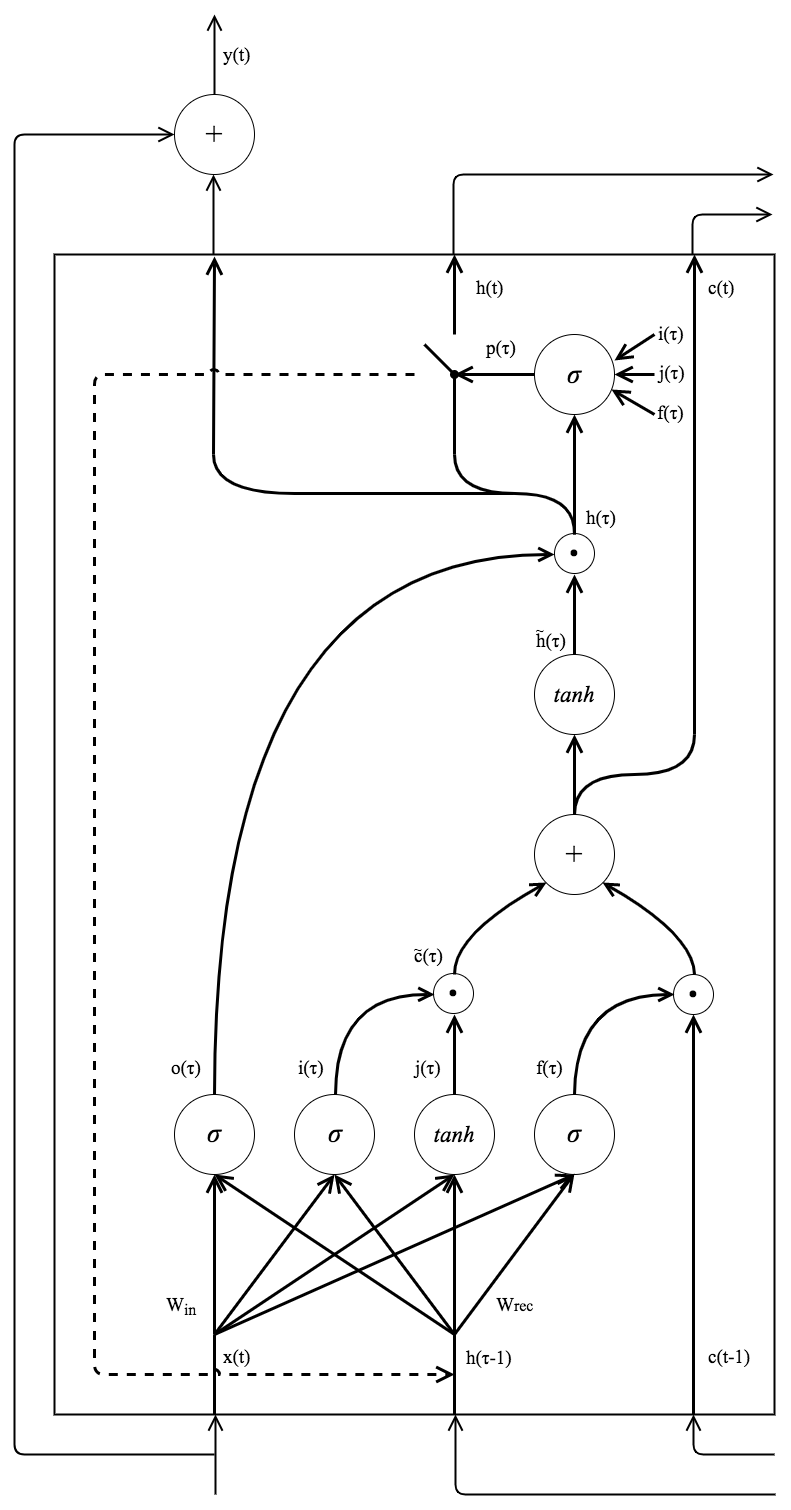
\includegraphics[scale=0.2]{iterativeLSTM.png}
		\caption{Flujo de información en cada iteración de la celda LSTM iterativa.}
		\label{iterativeLSTM}
	\end{figure}
	
	Cómo puede verse en la figura \ref{iterativeLSTM} la mayor parte de la estructura original de la celda LSTM se mantiene intacta. \\
	Por otro lado se incorpora la realimentación instantánea del estado de la celda entre iteraciones de forma explícita. La selección de exponer el estado de la celda obtenido en la iteración actual o realizar una nueva iteración realimentando el estado final de la celda obtenido en la iteración actual es realizada por una nueva regresión logística que en este caso se realiza sobre el estado $h(\tau)$ de la celda y los valores de las compuertas $i(\tau)$, $f(\tau)$ y la clasificación $j(\tau)$, al finalizar la iteración corriente.\\
	En el caso de que la compuerta $p(\tau)$ no supere el umbral impuesto en la iteración actual para una celda del bloque se decide preservar el estado de la misma al finalizar la iteración, se calcula la variable $y(t)$ y se expone la misma a las capas superiores.\\
	Este comportamiento fue resuelto en la implementación provista descartando los valores del vector de estado de la celda y reemplazándolos con los previos en cualquier iteración subsiguiente a la cual previamente el valor de la compuerta $p$ no superó el umbral correspondiente.\\
	En dicha implementación solo se expone el resultado del bloque de celdas cuando el valor de la compuerta $p$ de todas las celdas de todos los \textit{batches} esta por debajo del umbral previsto para la iteración actual. Sin embargo solo se permite que se reactive la iteración de celdas LSTM dentro de un mismo batch ó, como es equivalente por la arquitectura usada; dentro de un mismo bloque de celdas LSTM.\\
	Finalmente se adiciona el vector de valores de las variables de entrada al resultado de la iteración para referenciar el mismo respecto de los valores de entrada según indica el enfoque residual adoptado\cite{28ResidualLearning}.\\
	
	La compuerta $p$ sirve de controlador sobre la evolución del estado de la celda, seleccionando de forma autónoma si conservar el estado actual o modificar el mismo.\\
	Existen otros modelos donde se usa un componente separado como controlador del comportamiento de la RNN\cite{18DifferentiableNeuralComputer, 30NeuralTuringMachines, 31NeuralTuringMachinesRevised} pero en este caso la arquitectura del controlador fue acotada a una única capa de neuronas en favor de reducir la complejidad del modelo. \\
	Por otro lado, se considera que la extracción de la información relevante para la decisión de preservar o modificar el estado es realizada por las variables ya presentes en la celda LSTM. Recientes publicaciones que exploran la capacidad de modelos simples para proveer información relevante para la toma de decisiones motivaron esta decisión conservadora\cite{32WideDeepLearning}.\\
	
	Es concebible una modificación símil a la propuesta pero que contemple iteraciones sobre una RNN de longitud mayor a una capa, así como también es posible considerar un componente más complejo como controlador para la resolver la decisión de modificar o preservar el estado actual de la celda.\\
	Sin embargo, para la presente investigación se considero más relevante exponer el efecto de la modificación propuesta que explotar la mejora de desempeño conseguible con un modelo de tal complejidad.\\
	
	Vale la pena destacar que el estudio de la celda LSTM como un sistema dinámico y la posterior propuesta de realizar sucesivas iteraciones sobre valores constantes de las variables de entradas toman como hipótesis que el modelo es capaz de optimizar el conjunto de parámetros $\theta$ para que a través de la dinámica de la celda descrita en (\ref{iterativeLSTMdynamics}) posicione los puntos fijos del sistema de forma conveniente.\\
	Esta hipótesis permite a la celda LSTM iterativa superponer las cuencas de los atractores en distintos instantes de tiempo, asociándolos a la misma información. De esta forma se preserva la información entre las iteraciones realizadas en sucesivos instantes de tiempo.
	
	
	\subsection{Transformación iterativa residual}
	La formulación descrita en (\ref{iterativeLSTMformulation}) permite considerar el método iterativo desde otro punto de vista relacionado con la operación de la celda sobre los valores de entrada.\\
	Es posible apreciar en la formulación de la celda LSTM descrita en la sección \ref{sectionLSTM} que el estado previo de la celda $h(t-1)$ actúa como un sesgo en la activación de las variables $j$, $i$, $f$ y $o$, debido a que aporta un término constante que es función de el valor de la entrada $x(t)$ en el instante $t$. Este término desplazará la región del dominio de los valores de las variables de entrada para los cuales se produce la activación de las variables internas de la celda.\\
	Luego, el valor de la variable $h(\tau)$ varía en la ejecución de sucesivas iteraciones permitiendo al modelo explorar distintas regiones del dominio de las variables de entrada, evaluando la activación de las variables internas de la celda en cada uno de ellos. Se conjetura que esta exploración del dominio de los valor de las variables de entrada permite a las celdas la clasificación de patrones más complejos.\\
	La complejidad de los patrones presentes en el dominio de las variables de entrada dependerá de la tarea particular en la que se emplee el modelo propuesto. En la siguiente sección se exponen propiedades del espacio sobre el cual fue evaluado el modelo presentado.\\
	
	Por otro lado, la capacidad de la celda LSTM iterativa para explorar distintas regiones del dominio de las variables de entrada dependerá de valores del conjunto de parámetros $\theta$. Sin embargo, es sencillo imaginar un escenario para el cual los hiperplanos asociados a la clasificación realizada por las variables $j$ e $i$ tienen norma opuesta y la distancia entre los mismos, dada por $b_j - b_i$, define la región sobre la cual se produce el máximo de la activación de la nueva información $\tilde{c}(\tau)$, incorporada al estado interno de la celda en la iteración $\tau$. Entonces, considerando valores similares para el peso del estado $h(\tau-1)$ sobre la activación de las variables $j$ e $i$, variando el valor de la variable $h(\tau-1)$ se explorarán distintas regiones sobre la cual se produce la activación de $\tilde{c}(\tau)$. Esta exploración permitiría la clasificación de patrones no lineales como el conocido caso del problema XOR\cite{33TimeXORElman}.\\
	
	Finalmente, considerar el sistema dinámico descrito por la evolución de los estados de una RNN que aplica la modificación propuesta permite generalizar el efecto de realizar sucesivas evaluaciones sobre los mismos valores de entrada actualizando el estado interno de la red.\\
	Entonces, partiendo de la ya explorada identidad (\ref{recurrentStateCalculation}) y considerando el comportamiento del sistema dinámico en un entorno cercano al punto fijo atractor realizando sucesivas iteraciones se obtiene
	\begin{equation}\label{iterativeTransformation}
	\begin{split}
	h(\tau) &= \dfrac{\partial h(\tau -1)}{\partial \tau} + h(\tau -1)\\
	h(\tau) &= \sum_{i = 0}^{\tau} \dfrac{\partial h(\tau -1)}{\partial \tau} \, + h(0)\\
	h(\tau) &= \sum_{i = 0}^{\tau} \mathrm{J}_f(h^*) \, (h(i) - h^*) \, + h(t-1)\\
	h(\tau) &= \underbrace{\mathrm{J}_f(h^*)}_{ \mathbb{R}^{n \times n}} \, \underbrace{\sum_{i = 0}^{\tau} \, (h(i) - h^*)}_{\mathbb{R}^{n \times 1}} + h(t-1)\\
	h(\tau) &= \mathrm{J}_f(h^*) \, \underbrace{\mathrm{H(t)}}_{\mathbb{R}^{n \times \tau }} \, \underbrace{\mathrm{P(t)}}_{\mathbb{R}^{\tau \times 1 }} + h(t-1)\\
	\end{split}
	\end{equation}
	donde $\mathrm{H(t)}$ es una matriz tal que su $j$-ésima columna se compone de los términos $h(j) - h^*$ correspondiente a la iteración $j$. Esta matriz expande el espacio vectorial original $\mathcal{V} \in \mathbb{R}^n$ correspondiente a los estados posibles de la celda en el instante $t-1$ a un espacio vectorial $\mathcal{K} \in \mathbb{R}^{n \times \tau}$ correspondiente a la evolución de estados posibles de la celda luego de $\tau$ iteraciones.
	$P(t)$ es una matriz cuya $i$-ésima fila pondera la variación producida en el estado del sistema en la iteración $i$. Esta matriz incorpora las posibles dependencias explícitas respecto del tiempo de la dinámica del sistema descrita en (\ref{recurrentStateCalculation}). \\
	En la estructura propuesta esta matriz se corresponde con la ponderación realizada por la compuerta $p(i)$ en la $i$-ésima iteración. Como las ponderaciones realizadas se aplican sobre cada celda, la matriz resultante es el producto de dos matrices donde la primera pondera cada coordenada del vector de estado de la red correspondiente a la salida de cada celda y la segunda sumariza estas variaciones obtenidas en cada iteración en una única dimensión correspondiente a la coordenada del vector del estado final de la celda en el instante $t$.\\
	
	Por otro lado, es oportuno destacar que si bien la implementación de la modificación propuesta sólo explora una ponderación producida por un componente externo sobre los estados intermedios de la evolución del estado de la red, esta ponderación también está sujeta a las dependencias explícitas del sistema dinámico respecto de la iteración realizada. Por lo tanto, es concebible una ponderación mas compleja de los estados intermedios de la celda producida por un componente externo de mayor envergadura o una dinámica del sistema con dependencias explícitas respecto de la iteración realizada.\\
	
	Adicionalmente, es importante mencionar que el número de iteraciones consideradas por el valor $\tau$ se corresponde con el máximo número de iteraciones realizables por el sistema y no esta limitado por las $k(t)$ iteraciones efectivamente realizadas en un instante $t$ particular. Sin embargo, es consistente argumentar que las iteraciones no realizadas no aportan información alguna.\\
	En la implementación de la modificación propuesta el numero $k(t)$ de iteraciones realizadas en el instante $t$ dependerá de la activación de la compuerta $p$, donde $p(l) = 1$ para todas las iteraciones $l$ tal que $l \le k$, indicando participación total en la sumatoria y $p(l) = 0$ para todas las iteraciones $l$ tal que $k < l \le \tau$, indicando que no participan de la sumatoria.\\
	En esta implementación el valor de $\tau$ está dado por el parámetro \texttt{max\_it}.
	
	La transformación iterativa expuesta en (\ref{iterativeTransformation}) indica que realizar sucesivas iteraciones evaluando el sistema dinámico descrito por la evolución del estado de una RNN cuyos valores de entrada son constantes equivale a realizar una transformación no lineal sobre un espacio vectorial aumentado en $\tau$ veces la cantidad de dimensiones original, siendo $\tau$ el número de iteraciones realizadas.\\
	El resultado de la transformación iterativa propuesta dependerá, según lo visto anteriormente, tanto del vector de estados $h$ en el instante $t-1$ como de los valores de entrada en el instante $t$. Por lo tanto es posible considerar esta transformación no lineal como dependiente de ambos vectores según
	\begin{equation*}
	h(\tau) = \underbrace{\mathrm{J}_f(h^*)}_{W} \, \underbrace{\mathrm{H(t)} \, \mathrm{P(t)}}_{\varphi(x(t), h(t-1))} + h(t-1)
	\end{equation*}
	donde $\varphi$ es una transformación no lineal del espacio vectorial de estados original de la celda $\mathcal{V} \in \mathbb{R}^n$ a un espacio vectorial $\mathcal{K} \in \mathbb{R}^{n \times \tau}$. $W$ es una matriz de pesos que pondera el resultado de la transformación $\varphi$.\\
	Considerando que se satisfacen las condiciones del teorema \ref{iterativeLSTMConvergenceTheorem} y la evolución del estado de la celda converge hacia el punto fijo atractor correspondiente a la cuenca en la que se encontraba el estado al momento de realizar las iteraciones, es posible considerar el efecto fuera del entorno cercano del punto fijo y reescribir (\ref{iterativeTransformation}) en favor de la generalidad como
	\begin{equation*}
	h(\tau) = W \, \varphi(x(t), h(t-1)) + h(t-1)
	\end{equation*}
	este resultado indica que la matriz $W$ se corresponde con un hiperplano sobre el espacio vectorial $\mathcal{K}$ que aumenta al espacio vectorial $\mathcal{V}$ a partir de aplicar la transformación no lineal $\varphi$. Este resultado puede ser interpretado como la aplicación de una función kernel\cite{46MLKernel} que actúa sobre la información presente en la red en el instante $t-1$ y la información presente en los los valores de las variables de entrada en el instante $t$.\\
	Por ultimo, considerando la modificación residual explorada en la sección \ref{sectionLSTM} el resultado de la evaluación de la RNN iterativa en el instante $t$ será
	\begin{equation*}
	y(t) = h(\tau) + x(t)
	\end{equation*}
	\begin{equation}
	y(t) = W \, \varphi(x(t), h(t-1)) + h(t-1) + x(t)
	\end{equation}
	Sobre este resultado es posible apreciar el valor $y(t)$ de la celda en el instante $t$ como una clasificación no lineal sobre un espacio vectorial aumentado\cite{47NonlinearClasification} con una referencia a los valores originales de las variables $h$ y $x$ a clasificar\cite{28ResidualLearning}.
	
	\pagebreak
	
	\section{Modelado del lenguaje}\label{sectionLanguageModeling}
	En esta sección se introduce el problema de modelado del lenguaje abordado en los experimentos y se mencionan aplicaciones destacables de RNN sobre el campo de NPL. El campo de NPL dentro de las ciencias de la computación y la inteligencia artificial concierne a múltiples tareas estrechamente relacionadas con las formas de representación del lenguaje y el modelado de los conceptos expresados por el mismo. \\
	Un conjunto de tareas destacables del campo de NPL lo constituye la generación artificial de textos, traducción automática, reconocimiento del habla, entendimiento del lenguaje natural y clasificación automática de textos. Luego de introducir la tarea de modelado del lenguaje se expondrán varias de sus aplicaciones tanto en tareas del campo de NPL como en otros campos.\\
	
	Las soluciones a las tareas mencionadas son comúnmente implementadas como un mapeo de una secuencia de entrada a una secuencia de salida aprovechando el orden característico del lenguaje modelado. Este procesamiento secuencial ha visto un gran avance en términos de desempeño a partir del uso de NNs y, particularmente, RNNs.\\
	Sin embargo, muchas de estas tareas se definen sobre dominios de datos de entrada constituidos por texto y el procesamiento de este dominio de entrada no está definido para las RNN, por lo que el primer problema a resolver es la transformación de los datos de entrada en secuencias de puntos $x(t) \in \mathbb{R}^n$.\\
	Existen muchos métodos distintos para obtener representaciones vectoriales de datos textuales; más adelante en esta sección se explora uno de los más difundidos.\\
	
	Habiendo resuelto la compatibilidad de la secuencia de entrada con el procesamiento realizado por las RNN es posible usar las mismas para mapear la secuencia de entrada a la secuencia de salida esperada. La aplicación de RNNs para modelar características del lenguaje objetivo será explorada más adelante en esta sección.\\
	
	Luego, existe una problemática simétrica a la obtener representaciones vectoriales de los datos de entrada y consiste en definir como el resultado de la RNN se corresponde con la secuencia de salida.\\
	Esto es comúnmente resuelto a partir de la concatenación de una capa de clasificación que seleccione la clase más probable de un conjunto de candidatas en base a la salida provista por la red. Usando este patrón ya estudiado en la sección \ref{sectionRNN}, se definen como clases candidatas a los símbolos del vocabulario de salida, sobre el cual se selecciona el más probable como salida del modelo.\\
	
	En el desarrollo restante de este documento se referencia a las palabras del lenguaje origen y a las palabras del lenguaje objetivo como símbolos. Esta denominación permitirá conservar la generalidad respecto de otros enfoques que consideran como símbolos a otras agrupaciones como $n$-gramas o caracteres. En los casos en los que se mencione el vínculo de los símbolos con un concepto al que referencia se debe considerar que es posible que no existe un único concepto asociado al símbolo como en el caso de los caracteres.\\
	
	Pudiendo obtener la predicción del siguiente símbolo realizada por el modelo, se evalúa la misma midiendo a las propiedades de la distribución predicha por el modelo sobre todos los posibles símbolos del lenguaje objetivo, para cada instante de la secuencia de salida. \\
	Una métrica comúnmente usada para determinar el desempeño del modelo es la \textit{perplejidad} por palabra. Esta métrica puede interpretarse como la cantidad de clases que el modelo considera igualmente viables como alternativas para el valor del siguiente símbolo $y(t)$ de la secuencia de salida.\\
	El cálculo de la perplejidad por palabra del modelo sobre el símbolo $y(t)$ de la secuencia de salida en el instante $t$ es el siguiente
	\begin{equation*}
	PPL(p)=2^{H(p)} = 2^{-\sum_{y} p(y(t))\log p(y(t))}
	\end{equation*}
	donde $H(p)$ es la entropía de la distribución modelada $p$. La sumatoria recorre todos los símbolos posibles de la secuencia de salida que se corresponde con los símbolos del lenguaje objetivo.\\
	
	Finalmente se optimiza el conjunto de parámetros $\theta$ del modelo para minimizar la perplejidad por palabra sobre el set de entrenamiento. Se considera que la distribución de símbolos presente en el set de entrenamiento es una buena aproximación de la distribución sobre el set de test que no es accesible para el modelo al momento del entrenamiento.\\
	
	En la práctica se busca que la distribución modelada coincida con la distribución de secuencias de salidas asociado al lenguaje objetivo. \\
	Teniendo en cuenta que no se conoce explícitamente la distribución $p$ que se busca modelar (de otra forma la tarea estaría resuelta) se acota superiormente la misma\cite{34JurafskyBook}, aplicando el teorema Shannon-McMillan-Breiman, por la entropía cruzada de la distribución $y(t)$ expuesta por el modelo y la probabilidad del siguiente símbolo esperado, presente en el set de entrenamiento, para obtener una señal de error durante el entrenamiento del modelo.\\
	
	La distribución de probabilidad del siguiente símbolo concentra toda la probabilidad para el símbolo que se espera que prediga el modelo y que es extraído directamente del set de entrenamiento.\\
	Por lo tanto la entropía cruzada para la distribución del modelo y la distribución del siguiente símbolo es igual a la divergencia Kullback-Leibler\cite{63WordEmbeddingTyingTheory}, por lo que en cada variación de los parámetros realizada para optimizar el valor de la función objetivo se busca reducir la discrepancia entre las distribuciones mencionadas.\\
	En Inan et.al(2016)\cite{63WordEmbeddingTyingTheory} se propone una generalización del esquema de entrenamiento basados en este resultado. En este esquema de entrenamiento se calcula una distribución de símbolos esperados que sean similares al símbolo efectivamente hallado en el set de entrenamiento. \\
	El efecto obtenido al aplicar el framework propuesto es el de optimizar el conjunto de parámetros para reducir la discrepancia entre la distribución predicha y la distribución de ocurrencia de todos los símbolos considerados similares al símbolo efectivamente hallado en el set de datos. Más aún, el símbolo hallado en el set de datos constituirá el valor medio de la distribución objetivo que se intentará aproximar en cada variación de los parámetros producida por cada muestra extraída del set de entrenamiento.\\
	
	El framework mencionado es fácilmente implementable en la tarea de modelado del lenguaje debido a que se dispone de una distribución intuitiva sobre los símbolos que comparten la probabilidad de ser seleccionados. Esta distribución de símbolos esperados es obtenida como la proyección al espacio embebido del símbolo esperado, extraído del set de datos, seguido de la posterior proyección de la representación en el espacio embebido hacia el espacio de símbolos del lenguaje objetivo. \\
	En otras tareas la selección de la distribución de clases similares a la actualmente encontrada en el set de entrenamiento puede no ser tan intuitiva y requerir de algún conocimiento del dominio.\\
	
	Es oportuno destacar que en las primeras evaluaciones de la función objetivo la misma podría no proveer ninguna señal informativa para el entrenamiento bajo el framework mencionado. Según los autores del framework esta situación debería revertirse al progresar el entrenamiento obteniendo señales de actualización incrementalmente más informativas que las distribuciones de los símbolos efectivamente encontrados en el set de entrenamiento.
	
	\subsection{Espacios embebidos de palabras}
	La tarea de obtener representaciones vectoriales de datos textuales es un tópico ampliamente estudiado\cite{35MikolovRecurrentEmbeddings} debido a su importancia para las tareas del campo NLP.\\
	La cantidad de modelos que requieren representaciones vectoriales ha aumentado recientemente y este aumento fomento el desarrollo de métodos que provean representaciones vectoriales más eficaces\cite{36MikolovImprovement}.\\
	
	Una solución inicial al problema de tener una representación vectorial universal de los símbolos del lenguaje de entrada es la de codificar los mismos en vectores cuyas dimensiones registren la presencia de cada uno de los símbolos posibles del lenguaje.\\
	De esta manera es posible representar un texto como una secuencia de vectores cuyas coordenadas son 0 excepto en la dimensión relacionada con el símbolo que representan donde tendrá un valor de 1. \\
	A diferencia de la codificación dada en forma de secuencias de vectores con una única dimensión distinta de 0, otra codificación posible para el texto es un único vector donde se registren en las respectivas coordenadas los símbolos presentes en el mismo. Esta codificación es conocida como \text{bag of words}.\\
	
	Las representaciones mencionadas tienen la característica de capturar la coocurrencia de símbolos, que es un aspecto fundamental bajo la hipótesis de que la coocurrencia de símbolos relaciona el significado de los mismos. Esta hipótesis considera que la frecuencia con la que los símbolos ocurren en un mismo texto es una medida de la similitud de su significado.\\
	Otra característica de estas representaciones es la de tener una gran dispersión ya que la mayoría de las dimensiones de los vectores involucrados tienen el mismo valor 0. Esta característica hace ineficiente su procesamiento ya que no es posible aplicar métodos de compresión usados sobre representaciones densas\cite{60TeoricCorrespondenceOfWordEmbeddings}.\\
	
	Recientemente, las generación de representaciones vectoriales tuvo un gran progreso debido a la inclusión de NNs en el cálculo de los vectores que representan cada símbolo del lenguaje de origen\cite{37BengioNeuralEmbedding, 38MikolovFormer, 39GlovePennington}.\\
	La difusión tardía de estos métodos es comúnmente atribuida a los requerimientos de capacidad computacional prohibitivos para los investigadores en años pasados.\\
	
	El método para obtener una representación generada por modelo neuronal consiste en tomar como entrada la representación dispersa discutida anteriormente, dada por un vector cuyas dimensiones se corresponden con cada símbolo posible del lenguaje de origen y tiene valor 1 para la dimensión del símbolo a representar y 0 en otro caso, y buscar la representación tabulada del símbolo a representar en el espacio embebido.\\
	Los parámetros del modelo son previamente optimizados tareas no supervisadas donde se incorporan NNs que reciban como entrada las representaciones embebidas para inferir la presencia de otros símbolos en un contexto cercano. \\
	La optimización sobre la tarea de inferir la presencia de símbolos dado un contexto requiere que la relación entre los conceptos atribuidos a los símbolos se preserve en forma geométrica sobre el espacio embebido, lo cual en consecuencia mejora el desempeño de subsecuentes modelos que usen esta representación\cite{40CollobetWeston}.\\
	
	En modelos recientes la red neuronal dispone de funciones de activación lineales por lo que la inferencia se reduce a una multiplicación matricial. Esta decisión está fundada en la reducción de la complejidad computacional requerida.\\
	Es oportuno destacar que reducir la complejidad computacional del modelo, extrayendo las operaciones no lineales, acelera el entrenamiento de los parámetros ya que es posible calcular mas veces la variación en los parámetros indicada por el gradiente de la función objetivo. Es evidente entonces que existe una negociación entre complejidad del modelo y velocidad de entrenamiento.\\
	
	\subsection{Modelado del lenguaje usando NNs}
	El modelo neuronal del lenguaje propuesto en Bengio et.al (2003)\cite{37BengioNeuralEmbedding} usa las representaciones en el espacio embebido de las palabras presentes en un contexto cercano la palabra a predecir para el cálculo de la probabilidad para cada posible palabra obtenida de la evaluación de una NN sobre la que se aplica una capa softmax. Un esquema simplificado del modelo mencionado es expuesto en la figura \ref{nnModelLanguage}.\\
	Este modelo superó a los modelos tradicionalmente constituidos por el cálculo de la probabilidad de $N$-gramas y permitió considerar un contexto mas amplio al momento de realizar la inferencia de la palabra a predecir.\\
	
	\begin{figure}[H]
		\centering
		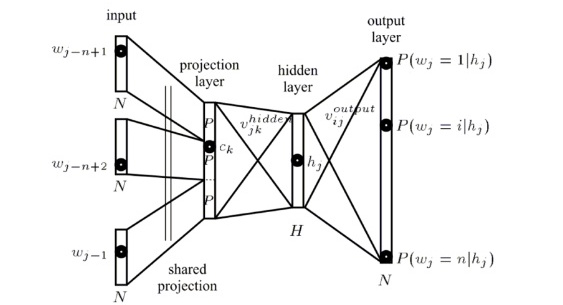
\includegraphics[scale=0.5]{nnLanguageModel.jpg}
		\caption{Bengio, Y., Schwenk, H., Sencal, J. S., Morin, F., \& Gauvain, J. L. (2006). 
			Neural probabilistic language models. In Innovations in Machine Learning (pp.137-186). Springer Berlin Heidelberg.}
		\label{nnModelLanguage}
	\end{figure}
	
	Profundizando el cálculo de la representación vectorial en el espacio embebido se reconoce una primera capa que multiplica la representación dispersa mencionada de los símbolos por una matriz de pesos. Esta primer capa, denominada \textit{embedding layer} o \textit{projection layer}, indexa las representaciones en el espacio embebido para cada símbolo, codificadas en las filas de la matriz de pesos obteniendo únicamente la representación del símbolo cuyo valor en la representación original es 1 a través de una simple multiplicación matricial.\\
	La matriz en cuestión tiene un tamaño proporcional al tamaño del vocabulario del lenguaje de origen y proporcional a la cantidad de \text{features} o dimensiones de la representación vectorial del espacio embebido de palabras. Estas representaciones presentes en la capa de proyección fueron originalmente denominadas \textit{distributed feature vectors}.\\
	Las representaciones de los símbolos obtenidas de la capa de proyección cumplen estar agrupadas de forma espacial según la similitud de los símbolos que representan. Esta característica surge de la propiedad de la función diferenciable modelada por la NN ya que la suavidad de la función usada para calcular la distribución de probabilidad requiere que cambios pequeños en los valores de entrada produzcan pequeñas variaciones en el resultado de la función. \\
	Por lo tanto, las representaciones de símbolos ``similares'', distribuidos muy próximos entre si en el espacio embebido, podrían ser igualmente plausibles como alternativas para el símbolo a predecir por su significado análogo deberán estar cercanos en el espacio vectorial de representaciones de palabras.\\
	
	La red neuronal mencionada constituye una capa superior, denominada \textit{hidden layer}, que demanda una capacidad comunicacional proporcional al tamaño del vector de features que representa cada símbolo del lenguaje de origen.\\
	Adicionalmente, es posible aumentar la cantidad de capas de neuronas concatenadas en la NN para obtener representaciones de los símbolos respecto de features más abstractas que faciliten la clasificación lineal por la capa softmax. Como efecto secundario esto incrementa la exigencia computacional del modelo.\\
	El objetivo de la NN es el de calcular la ocurrencia un conjunto de features más abstractas, denominadas \textit{hidden features} por no ser observables explícitamente en el set de datos. Estas features permiten representar al vector sobre un espacio vectorial de más alto nivel sobre el cual es posible aplicar una proyección al espacio de los símbolos propios lenguaje objetivo. Esta proyección es usada en conjunto con la función softmax para proveer una distribución de probabilidad válida.\\
	Formalmente, es posible considerar la probabilidad de cada símbolo del lenguaje objetivo como la ocurrencia de los valores adecuados de las features de abstractas provista por el resultado de la NN según
	\begin{equation}\label{featureWordProb}
	P(w_j = i | h_j) = \prod_{k=0}^{m}P(h_{j_k} = h_k(i)) \quad , \forall \, i \, \in V^{out}
	\end{equation}
	donde $w_j$ es el símbolo a predecir en el instante actual. El vector $h_j \in \mathbb{R}^m$ es el vector de valores de las features abstractas calculado por la NN en un instante dado y $h_{j_k} \in \mathbb{R}$ es el valor de su $k$-ésima coordenada. $V^{out}$ es el conjunto de símbolos del vocabulario propio lenguaje de destino que es recorrido para todos los símbolos $i$. $h_k(i) \in \mathbb{R}$ es el valor de la $k$-ésima feature asociado al símbolo $i$.\\
	Luego, tomando el logaritmo de la probabilidad \ref{featureWordProb} se obtiene
	\begin{equation*}
	\begin{split}
	\ln P(w_j = i | h) &= \ln (\prod_{j=0}^{m}P(h_{j} = h_j(i))) \\
	\ln P(w_j = i | h) &= \sum_{j=0}^{m} \ln (P(h_{j} = h_j(i))) = \sum_{j=0}^{m} v^{output}_{ij} \, h_{j} \\
	\ln P(w_j = i | h) &= v^{output}_i \, h  \quad , \forall \,i \, \in V^{out}\\
	\end{split}
	\end{equation*}
	donde $v^{output}_{ij}$ es la $j$-ésima coordenada de la fila $v^{output}_i$ de la matriz $v^{output}$ que proyecta los valores de las features abstractas calculadas por la NN al espacio de los símbolos propios lenguaje objetivo.\\
	Finalmente la capa softmax normaliza la salida de la proyección obtenida para exponer una distribución de probabilidad multinomial sobre los símbolos del vocabulario del lenguaje objetivo según
	\begin{equation}\label{logLinearFeatureModel}
	\begin{split}
	\ln P(w_j = i | h) &= v^{output}_i \, h  \quad , \forall \,i \, \in V^{out}\\
	e^{\ln P(w_j = i | h)} &= e^{v^{output}_i \, h}\\
	P(w_j = i | h) &\,\alpha\, e^{v^{output}_i \, h}\\
	P(w_j = i | h) &= \displaystyle\frac{e^{v^{output}_i \, h}}{\displaystyle\sum_{j \in V^{out}} e^{v^{output}_j \, h}} \quad , \forall \, i \, \in V^{out}
	\end{split} 
	\end{equation}
	De esta manera los valores de las features abstractas calculados por la NN son usadas para la selección del símbolo con mayor probabilidad de ocurrencia en el instante actual.\\
	Es posible apreciar en (\ref{logLinearFeatureModel}) que el cálculo de la probabilidad de cada símbolo requiere el cálculo de una constante en la que se recorre el vocabulario completo del lenguaje objetivo, por lo tanto la complejidad computacional de esta operación crece linealmente con el vocabulario del lenguaje objetivo.\\
	
	El modelo Word2Vec, recientemente publicado\cite{38MikolovFormer}, elimina la necesidad de la capa superior en favor de un modelo computacionalmente más simple. Este modelo fue publicado en conjunto con dos arquitecturas diferentes para su implementación denominadas \textit{Continuous Bag of Words}(CBOW) y \textit{Continuous Skipgram}(CSG).\\
	La arquitectura CBOW, expuesta en la figura \ref{word2Vec} (a), incorpora símbolos en un contexto que incluye tanto los símbolos previos al símbolo a predecir cómo los futuros, según el orden en el que suceden en la secuencia de entrada. Cada una de las representaciones de estos símbolos en el contexto del símbolo a predecir es promediada para producir la representación predicha.\\
	La arquitectura CSG, expuesta en la figura \ref{word2Vec} (b), considera únicamente un símbolo de la secuencia de entrada para predecir la presencia de los símbolos en un contexto de tamaño variable, acotado en cantidad de símbolos por un parámetro límite $C$.\\
	Ambas arquitecturas mencionadas realizan clasificaciones del tipo \textit{log-linear}, por lo tanto estas clasificaciones consisten de una regresión lineal sobre los valores de las variables de la capa de proyección en la escala logarítmica.\\
	
	\begin{figure}[H]
		\centering
		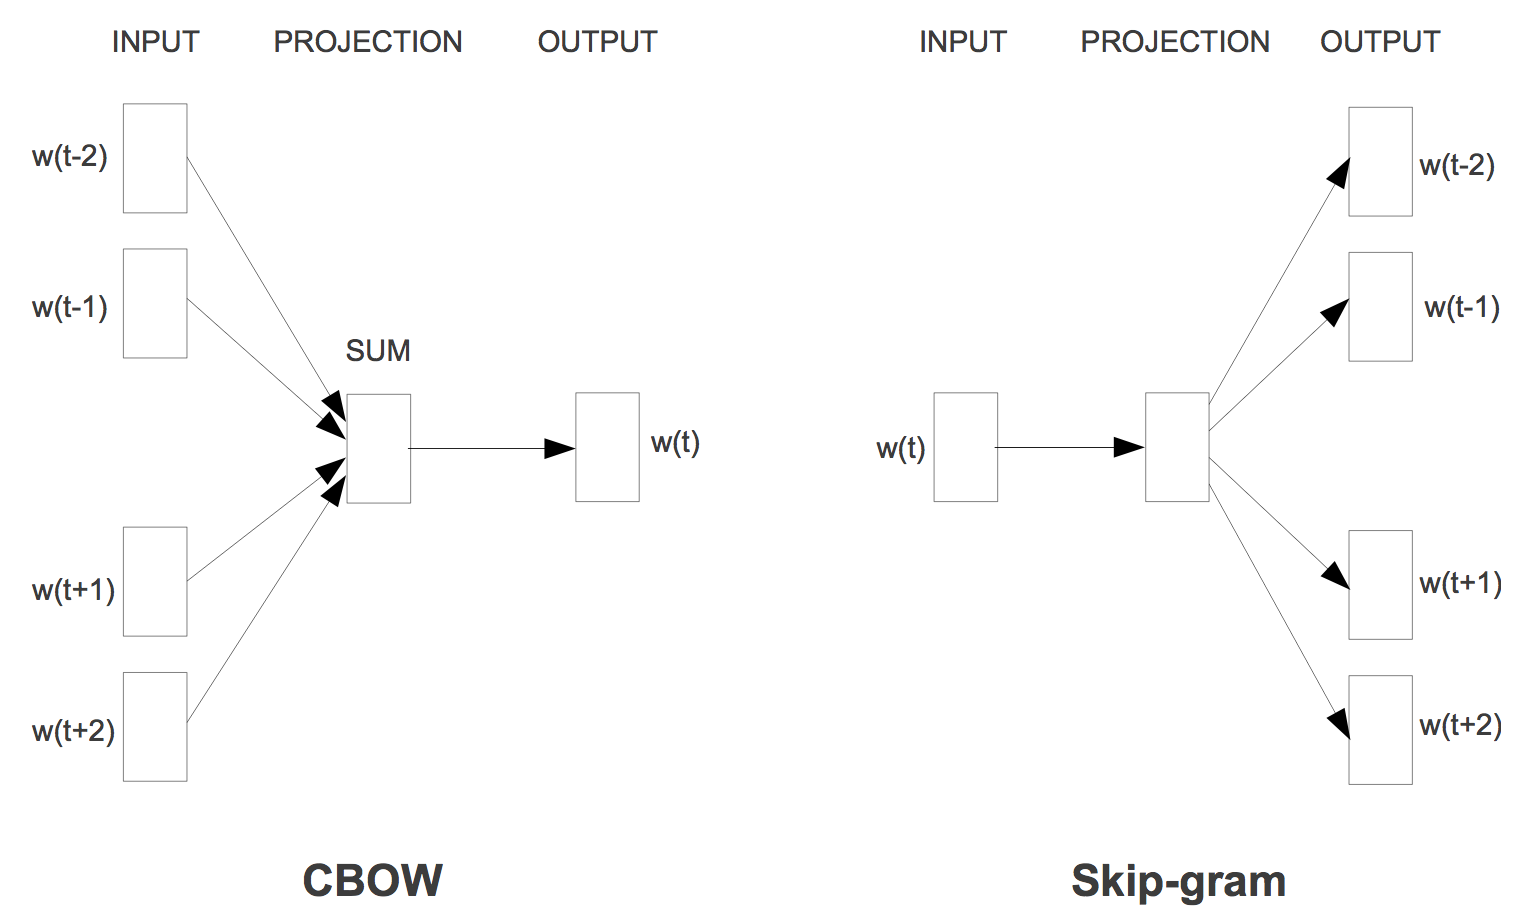
\includegraphics[scale=0.4]{word2Vec.png}
		\caption{Tomas Mikolov, Ilya Sutskever, Kai Chen, Greg Corrado, and Jerey Dean. Distributed
			Representations of Words and Phrases and their Compositionality. NIPS, 2013.}
		\label{word2Vec}
	\end{figure}
	
	Una serie de mejoras han sido propuestas por Mikolov y sus colegas con la intención de mejorar el desempeño del modelo Word2Vec, particularmente usando la arquitectura CSG\cite{36MikolovImprovement}.\\
	La primera modificación, denominada \textit{hierarchical softmax}, consiste derivar el extenso cálculo realizado en la clasificación sobre el espacio de contextos a la recorrida de una estructura arbórea. En concreto se calculan las probabilidades de que cada símbolo ocurra en el contexto del símbolo de entrada multiplicando las probabilidades almacenadas en los nodos de un árbol Huffman donde se agrupan los símbolos del lenguaje de origen según su frecuencia en el set de entrenamiento.\\
	Esta modificación busca reducir el impacto de la capa de clasificación final constituida por la función softmax introducida en la sección \ref{sectionRNN} y formalizada en (\ref{logLinearFeatureModel}), pasando de un orden lineal a un orden logarítmico respecto del vocabulario del lenguaje.\\
	Otra modificación introducida fue la penalización de contextos ajenos a cada símbolo. Esta penalización, denominada \textit{negative sampling}, se realiza muestreando $k$ símbolos como contextos de una distribución parametrizable de ruido y minimizando la probabilidad de que sean predichos por el modelo.\\
	Esta modificación mejora la calidad de las representaciones de los símbolos al dispersarlos respecto de los contextos menos probables.\\
	Una ultima modificación sobre la arquitectura original busca reducir el efecto de los símbolos más comunes del lenguaje ya que los mismos aportan poca información semántica. Para lograr esto se descarta la ocurrencia de un símbolo en el corpus de entrenamiento según una distribución de probabilidad que dependa de la frecuencia de dicho símbolo en el corpus. Típicamente esta distribución es parametrizable para que las ocurrencias de los símbolos con una frecuencia superior a un umbral tengan una alta probabilidad de ser descartadas.
	
	Por otra parte, otros modelo basados en el uso explícito de la coocurrencia de palabras han sido recientemente propuestos\cite{39GlovePennington}. Un modelo que se destaca por su desempeño es GloVe\cite{45WordEmbbedingComparison}. Este modelo considera las propiedades lineales del espacio embebido para factorizar el logaritmo de la matriz de coocurrencia de símbolos en el set de entrenamiento mediante la siguiente fórmula
	\begin{equation*}
	W(x_i)^T \, W(x_k) + b_i + b_k = \log(X_{ik})
	\end{equation*}
	donde $W(x)$ corresponde al vector que representa al símbolo $x$ del lenguaje origen en el espacio embebido. $b_i$ y $b_k$ son vectores de sesgos correspondientes a los símbolos $x_i$ y $x_k$ respectivamente. $X_{ik}$ es la coocurrencia de los símbolos $i$ y $k$. Los símbolos $x_i$ y $x_k$ se corresponden con todos los pares posibles de símbolos del lenguaje de origen y la simetría de la formulación del modelo indica que la relación entre los mismos se mantiene ya que cualquiera de los dos es contexto de otro.\\
	A pesar de que el la optimización de esta formulación está en principio acotada por un factor $|V|^2$, donde $|V|$ es el tamaño del vocabulario del idioma de origen, los autores estiman una cota superior comparable con la del modelo Word2Vec y proporcional al tamaño del corpus de datos.\\
	Como en el caso de los modelos mencionados anteriormente, las representaciones de los símbolos están codificadas en una matriz de pesos que es indexada por la representación dispersa del símbolo en el lenguaje de origen. En todos los casos esta matriz es optimizada haciendo uso del gradiente de la función objetivo correspondiente a cada modelo.\\
	Mientras que este modelo explícitamente considera la coocurrencia de símbolos en el corpus de datos, todos los modelos mencionados contemplan la ocurrencia conjunta de los símbolos como un indicio de la relación entre el significado atribuido a los símbolos del lenguaje de origen.\\
	
	La semejanza teórica entre los modelos expuestos fue abordada por Levy y Goldberg(2014)\cite{60TeoricCorrespondenceOfWordEmbeddings} donde se detalla matemáticamente como el método CSG con negative sampling optimiza los parámetros del modelo para obtener una aproximación a la matriz $M^{PMI}$ de punto de información mutua(PMI, por su siglas en inglés)\cite{61PointMutualInformation}.\\
	Esta matriz retiene en sus coeficientes los valores de la métrica de información mutua entre un símbolo y un contexto específico. Esta métrica es calculada en base a la ocurrencia parcial y conjunta de la símbolo y el contexto en el corpus de datos.\\
	Se encuentra en dicha publicación que el método presentado obtiene una factorización simétrica de la matriz PMI. La factorización en cuestión es densa y se compone de la multiplicación de las matrices propias de la capa proyección desde el lenguaje de origen y de la capa de proyección hacia el de contextos.\\
	
	Un ejemplo donde se expone la característica de preservación del significado en forma geométrica conseguida con el uso de los modelos presentados lo constituye la siguiente operación sobre el espacio embebido\\
	\begin{equation*}
	W(\texttt{'biggest'}) -W(\texttt{'big'})+W(\texttt{'small'}) \approx W(\texttt{'smallest'})
	\end{equation*}
	donde $W(x)$ corresponde al vector que representa al símbolo $x$ del lenguaje origen en el espacio embebido.\\
	Muchos ejemplos como este pueden ser generados operando con las representaciones de los símbolos del lenguaje de origen en el espacio embebido. Una serie de servicios web proveen esta facilidad\footnote{\texttt{https://code.google.com/archive/p/word2vec/}}\footnote{\texttt{https://nlp.stanford.edu/projects/glove/}}\footnote{\texttt{https://ronxin.github.io/wevi/}}.\\
	
	La incorporación de NNs en la tarea de modelado del lenguaje ha tenido mucho éxito sobre los modelos más tradicionales de $N$-gramas, incluso con la inclusión de información semántica por el método LSI\cite{37BengioNeuralEmbedding}. Sin embargo, los modelos ya expuestos en esta sección incorporan información de un contexto de tamaño acotado, lo que limita la información extraíble de la secuencia de símbolos de entrada a las dependencias temporales presentes en el contexto seleccionado.\\
	Es evidente entonces que el uso de modelos de secuencia que consideren el procesamiento de secuencias de longitud variable permitiría explotar la información presente en las dependencias temporales con símbolos fuera del contexto seleccionado.\\
	Para incorporar la información de los símbolos fuera del contexto seleccionado es propuesto por Mikolov et.al (2010)\cite{49RNNLanguageModel} el uso de RNNs que consideren las dependencias sobre una secuencia de símbolos de longitud variable. Dicha publicación explora el uso de una RNN de una única capa en el rol de hidden layer exponiendo resultados que indican una indudable mejora en el desempeño del modelo al considerar secuencias de símbolos de longitud variable. Este modelo es expuesto en la figura \ref{RNNLanguageModel}.\\
	
	\begin{figure}[H]
		\centering
		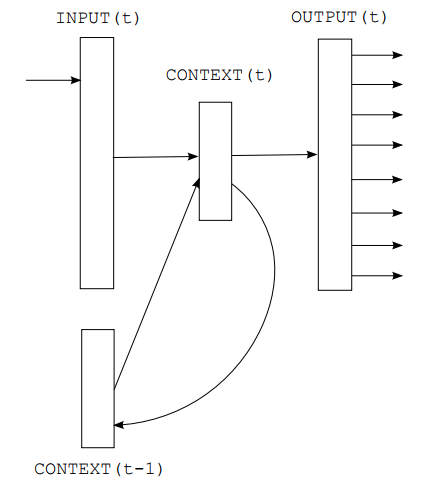
\includegraphics[scale=0.5]{RNNLanguageModel.png}
		\caption{Recurrent neural network based language model. Mikolov et al., Interspeech, ’10.}
		\label{RNNLanguageModel}
	\end{figure}
	
	Recientemente Press et.al(2016)\cite{53SharingInputAndOutputEmbeddings} ha explorado el vínculo entre las representaciones obtenidas en la capa de proyección desde el lenguaje origen y las obtenidas en la capa de clasificación softmax hacia el lenguaje destino. Este esquema también fue abordado en forma teórica y práctica por Inan et.al\cite{63WordEmbeddingTyingTheory}.\\
	Se encuentra en dicho análisis que compartir los parámetros entre la capa de proyección y la ultima capa de clasificación permite reducir la cantidad de parámetros a optimizar y conservar el desempeño de un modelo mucho más complejo en términos de cantidad de parámetros.\\
	Este resultado se relaciona con las observaciones de Liao et.al(2016)\cite{2BridgingGaps} ya que en ambos casos se encuentran beneficios al reutilizar los parámetros del modelo.\\
	En el presente trabajo se considera la reutilización de parámetros como una evaluación iterativa por lo que el trabajo realizado sobre la reutilización de los parámetros de las capa de proyección desde el lenguaje origen y hacia el lenguaje objetivo se relaciona tangencialmente con el trabajo presentado.
	
	\subsection{Aplicaciones del modelado del lenguaje}
	La tarea de modelado del lenguaje constituye una de las aplicaciones de aprendizaje no supervisado más exitosas conocidas. Los modelos del lenguaje obtenidos al optimizar la función objetivo preservan la relación semántica de los símbolos presentes en el vocabulario del lenguaje usado.\\
	Es interesante destacar que los modelos del lenguaje son entrenados sobre conjuntos de datos no categorizados manualmente. El único requerimiento de los modelos mencionados, respecto de los datos de entrenamiento, es el disponer de una colección de textos de los cuales puedan extraer de forma autónoma las relaciones entre los conceptos atribuidos a los símbolos del lenguaje de origen.\\
	Esta facilidad de usar datos de entrenamiento que no requieran de una intervención manual es una característica importante debido a que la obtención de datos de entrenamiento categorizados manualmente suele ser un proceso difícil y costoso, ademas de sesgar la precisión de los mismos al desempeño humano. \\
	Es concebible entonces el uso de modelos del lenguaje sobre amplios conjuntos de datos textuales relacionados con una tarea a resolver que permitan extraer conocimiento semántico sobre la misma de forma automática.\\
	A diferencia de los conjuntos de datos de entrenamiento categorizados manualmente, los corpus de datos usados para entrenar modelos del lenguaje son accesibles fácilmente y de forma gratuita.\\
	Embeber modelos del lenguaje dentro de modelos usados para otras tareas permite entonces ganar una intuición semántica sobre la descripción interna procesada a partir de proyectar la misma a símbolos reconocibles. Tienen además el potencial de extraer conocimiento de datos no categorizados manualmente de forma automática.\\
	
	La aplicación de modelos del lenguaje en tareas de visión computarizada\cite{43ParsingScenesRecursively, 48WordImageEmbedding} vincula las imágenes procesadas por un modelo visual con las representaciones en el espacio embebido de palabras de los símbolos que referencian a los objetos en la imagen de entrada. De esta manera es posible obtener descripciones generadas de forma autónoma por el modelo del lenguaje entrenado.\\
	Análogamente, la aplicación de modelos del lenguaje permite la sintetización de imágenes realistas en base a descripciones textuales de la misma\cite{50StackGANs}.\\
	
	En la tarea de traducción automática la aplicación de modelos del lenguaje permite codificar las palabras del lenguaje original del texto a traducir, para a continuación decodificarla en una o más palabras del lenguaje destino al que se intenta traducir el texto \cite{51SequenceToSequenceMachineTranslation, 52MachineTranslationAttentionRNN}. Esta operación se realiza a través de modelar la función de correspondencia de la representación en el espacio embebido de palabras del lenguaje original con la representación en el espacio embebido de palabras del lenguaje destino.\\
	Se destaca también la importancia de las RNNs en los modelos con mejor desempeño en esta tarea.\\
	
	Respecto a la tarea de reconocimiento del habla, la inclusión de modelos del lenguaje fortaleció el desempeño de los modelos a partir de incluir una medida de la coherencia de cada transcripción alternativa generada por modelos de audio\cite{54SpeechRecognitionLMLatticeScoring, 55WordEmbeddingsRescoringSpeechRecognition, 56MicrosoftSpeechRecognition}.\\
	La inclusión de modelos de lenguaje se realiza puntuando una lista de $N$ mejores alternativas previamente puntuadas por un modelo acústico. El modelo del lenguaje provee entonces un nuevo puntaje considerando la verosimilitud de las $N$ alternativas obtenida del logaritmo de la distribución de probabilidad sobre la que se entrenó el modelo del lenguaje.\\
	Los resultados obtenidos aplicando modelos del lenguaje exhiben mejoras apreciables en la coherencia de las transcripciones efectuadas.\\
	
	Dentro de la tarea de análisis de sensibilidad y clasificación de documentos los modelos del lenguaje constituyen un componente fundamental para el cálculo de la probabilidad de que una expresión pertenezca a una categoría.\\
	En este contexto las representaciones de los símbolos del lenguaje son usadas como valores de las variables de entrada a modelos, usualmente NNs, que infieran la pertenencia del texto a un conjunto de clases.\\
	Los modelos del lenguaje que preservan el contenido semántico de los símbolos procesados permiten extraer los conceptos presentes en la secuencia original para finalmente utilizar un modelo específico de la tarea a realizar para establecer la correspondencia de la secuencia de símbolos con una conjunto de clases objetivo\cite{57SentimentAnalysisLanguageModels}.\\
	
	En la tarea de recuperación de información los modelos del lenguaje permiten analizar las consultar realizadas como colecciones de símbolos del lenguaje original para extraer representaciones en un espacio vectorial al cual previamente fueron mapeados los documentos de una colección\cite{58WordEmbeddingInformationRetrieval}. Esto posibilita encontrar en el mencionado espacio los documentos más próximos a la consulta realizada en términos de relevancia semántica\cite{59RelevanceWordEmbeddings}.
	
	Los modelos del lenguaje también son ampliamente usados en la tarea de sumarización de textos debido a su facilidad para extraer información semántica de la secuencia original.\\
	En los modelos de sumarización de textos las palabras del texto original son representadas en el espacio embebido de palabras para luego ser usados en un modelo más complejo que genere símbolos de la secuencia de salida, interpretada como el resumen del texto original\cite{64WordEmbeddingTextSumarization}.\\
	Algunos de estos modelos incorporan mecanismos para referenciar símbolos del texto original, evitando el problema de exponer símbolos no contemplados en el vocabulario al momento de construir el espacio embebido\cite{65WordEmbeddingTextSumarizationPointingBack}.\\
	
	No se puede ignorar que la inclusión de los modelos del lenguaje dentro de otros modelos para la resolución de tareas específicas es solo una pieza de un mecanismo más complejo y que los resultados obtenidos surgen de la colaboración de múltiples componentes.\\
	Por otro lado, es evidente que la aplicación del modelado del lenguaje en las tareas mencionadas provee una forma de vincular una representación interna de un modelo propio de una tarea específica con una representación en el espacio embebido de palabras. Esta representación es usada para reconstruir los símbolos correspondientes a los conceptos que expresan el elemento propio de la tarea en un lenguaje objetivo fácilmente reconocible.
	
	\pagebreak
	
	\section{Experimentos}\label{sectionExperiments}
	En esta sección se expondrán los resultados de los experimentos ejecutados aplicando la mejora propuesta y el efecto de variar los parámetros de la misma.\\
	La implementación de los experimentos y el modelo propuesto se basó en la implementación provista por la librería de machine learning, Tensorflow. Por otra parte, esta implementación está basada en la investigaciones previas\cite{14RegularizationZaremba}.\\
	
	Con el objetivo de exponer la mejora en el desempeño obtenida al implementar la modificación propuesta sobre la celda LSTM se realizaron experimentos sobre la tarea de modelado del lenguaje.\\ Los experimentos ejecutados inicializan una arquitectura de RNN explorada originalmente en Zaremba et.al(2014)\cite{14RegularizationZaremba}, aplican la modificación propuesta y varían los valores de los parámetros inherentes a la modificación realizada para exponer su efecto en el desempeño. Dicha publicación fue usada como referencia para todas las decisiones relacionadas a la configuración de los experimentos realizados.\\
	
	La tarea que es ejecutada con la intención de optimizar el conjunto de parámetros $\theta$ el modelo es la ya descrita tarea de modelado del lenguaje. En la misma se predice el siguiente símbolo presente en una secuencia de símbolos extraída de un corpus de texto. En todos los experimentos los símbolos considerados son palabras del idioma inglés.\\
	Se uso como implementación inicial del entrenamiento del modelo y ejecución de la tarea el código liberado junto con la librería Tensorflow\footnote{Código disponible para descargar en \texttt{https://github.com/tensorflow/models/tree/master/tutorials/rnn/ptb}.}.
	
	El corpus de datos usado para el entrenamiento del modelo es Penn Treebank\cite{41PennTreebankMarcus}\footnote{Corpus disponible para descargar en  \texttt{http://www.fit.vutbr.cz/~imikolov/rnnlm/simple-examples.tgz}.}. El tamaño del vocabulario usado se corresponde con las 10000 palabras más frecuentes en el corpus original y un <unk> token para considerar las palabras fuera del vocabulario especificado. El set de datos consiste en 929 mil palabras de entrenamiento, 73 mil palabras de validación y 82 mil palabras de prueba.\\
	Los símbolos extraídos de este set de datos son representados en un espacio embebido mediante la indexación de una matriz de pesos y dicha representación es usada como valores de las variables de entrada del modelo neuronal recurrente. \\
	
	La arquitectura usada para los experimentos realizados consiste en la generación de representaciones en un espacio embebido para el símbolo del instante actual de la secuencia de entrada $x(t)$ y su uso como valores de las variables de entrada de una o más capas de un bloque de celdas LSTM iterativas. Finalmente una capa softmax realiza la clasificación sobre los posibles símbolos del vocabulario para resolver la predicción del siguiente símbolo $x(t+1)$ de a secuencia de entrada.\\
	Luego de cada capa constituida por un bloque de celdas LSTM se aplica el método de regularización Dropout descrito en la sección \ref{sectionLSTM}. La probabilidad de descartar una conexión usando el método Dropout es de 0.5\\
	El modelo explora secuencias de símbolos realizando 35 evaluaciones sobre los subsecuentes símbolos presentes en el set de datos. Los estados iniciales de las RNNs son configurados al origen de coordenadas del espacio de estados al iniciar cada nueva secuencia.\\
	
	Los parámetros del modelo son optimizados usando el método minibatch gradient descent\cite{62MinibatchGradientDescent}. El tamaño de \textit{minibatch} usado es 20.\\
	Inicialmente los parámetros del modelo son inicializados usando una distribución uniforme en el intervalo $[-0.05, 0.05]$
	
	La cantidad de parámetros del modelo está determinada por la suma de la cantidad de parámetros requeridos por la capa de proyección al espacio embebido de símbolos y por la suma de parámetros de la RNN. \\
	Los parámetros en la capa de proyección dependen de la cantidad de celdas por bloque de celdas LSTM, ya que la dimensión del espacio embebido de palabras es tomada igual a cantidad de celdas presentes en la primera capa de la RNN, y por el tamaño del vocabulario usado.\\
	Los parámetros de la RNN son proporcionales a la cantidad de capas y la cantidad de celdas presentes en cada bloque de celdas LSTM. Por simplicidad se usan los mismos tamaños de bloque en todas las capas.\\
	
	El régimen de entrenamiento consiste en un valor de \textit{learning rate} $\alpha$ igual a 1 por las primeras 6 iteraciones, luego de las cuales el mismo es reducido por un factor de 1.2 por cada epoch. Se ejecutan en total 39 epochs de entrenamiento.\\
	
	Los resultados expuestos en la Tabla \ref{tableExperimentPerformance} muestran que los modelo que incorporan la modificación propuesta mejoran el desempeño respecto del modelo original, incluso en el caso de modelos considerablemente más simples en términos de cantidad de parámetros. \\
	El desempeño es medido por la perplejidad por palabra, como se adelantó en la sección \ref{sectionLanguageModeling}. Según esta métrica, los modelos con mejor desempeño tienen un valor menor de perplejidad.\\
	Los resultados tabulados corresponden a modelos optimizados como parte de la presente investigación, a excepción del modelo con mayor cantidad de parámetros para el cual se extrae la métrica de desempeño de su publicación original\cite{14RegularizationZaremba}.\\
	\begin{center}
		Tabla 1: Perplejidad por palabra en el set de datos Penn Treebank.\\
		
		\begin{tabular}[t]{| c  | c | c |}
			\hline
			Modelo & Tamaño & Perplejidad Test Set\\
			\hline
			\hline
			LSTM & 16M  & 84.48\\
			\hline
			LSTM iterativa & 16M  & 78.46\\
			\hline
			\hline
			LSTM(2 capas) & 20M  & 83.25\\
			\hline
			LSTM iterativa(2 capas) & 20M  & 78.60\\
			\hline
			\hline
			LSTM(2 capas)& 50M & \textbf{78.29}\\
			\hline
		\end{tabular}
		\label{tableExperimentPerformance}
	\end{center}
	
	Los resultados expuestos en la tabla \ref{tableExperimentPerformance} evidencian la competitividad de los modelos entrenados con modelos conocidos y de una cantidad de parámetros mayor. En concreto se encuentra una reducción mayor a \%300 en la cantidad de parámetros total del modelo sin una pérdida considerable en el desempeño.\\
	
	Para los modelos presentados no fue posible extraer métricas claras del tiempo de entrenamiento requerido, debido principalmente a que no se dispuso de recursos dedicados exclusivamente para la presente investigación. Sin embargo, es oportuno destacar que cualitativamente el tiempo requerido para entrenar el modelo aumenta proporcionalmente al total de iteraciones producidas por los bloques de celdas LSTM iterativas en el modelo.\\
	
	Con la finalidad de exponer el efecto en el desempeño sobre modelo original al variar la cantidad de iteraciones realizadas se entrenaron dos series de modelos con una arquitectura y cantidad de parámetros idéntica pero fijando las iteraciones realizadas en una cantidad incremental. La primer serie de modelos cuenta con una única capa de celdas LSTM iterativas y la segunda serie cuenta con dos capas de celdas LSTM iterativas. Los parámetros de entrenamiento se mantuvieron constantes entre estos modelos.\\
	
	La configuración del experimento es la ya mencionada en esta sección para la comparación con modelos mas complejos, a excepción que en este experimento se fuerza la cantidad de iteraciones a realizar eliminando así la necesidad del controlador que regula la ejecución de futuras iteraciones.\\
	La figura \ref{pplVsIterationsFigure} expone los resultados obtenidos para las dos series de modelos entrenados. En dicha figura puede verse como aumentar las iteraciones mejora apreciablemente el desempeño del modelo independientemente de la complejidad del mismo vinculada a la cantidad de capas de la RNN.
	\begin{figure}
		\centering
		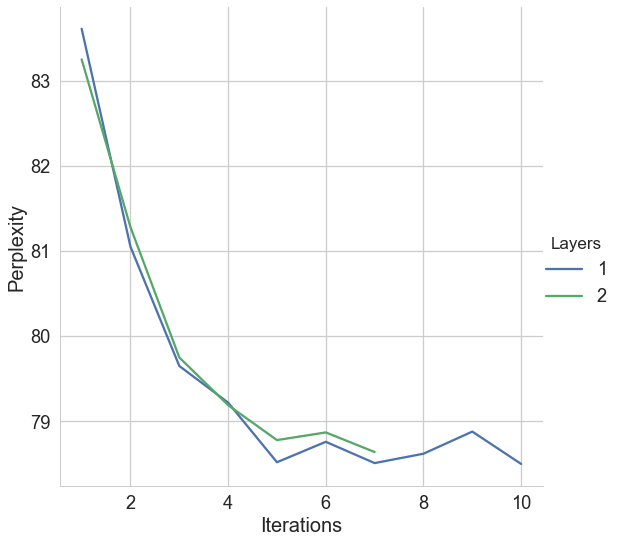
\includegraphics[scale=0.4]{pplVsIterations.png}
		\caption{Perplejidad por palabra en función de las iteraciones realizadas.}
		\label{pplVsIterationsFigure}
	\end{figure}
	
	Como puede observarse en la figura \ref{pplVsIterationsFigure} el desempeño del modelo mejora consistentemente al aumentar la cantidad de iteraciones realizadas. Adicionalmente, se evidencia que un modelo simple de una única capa obtiene un mejor desempeño que su versión más compleja con mayor cantidad de capas al aumentar la cantidad de iteraciones realizadas mas alla del tradicional esquema de una única iteración.\\
	
	Es oportuno observar que la figura \ref{pplVsIterationsFigure} indica que la mejoría en el desempeño del modelo expuesta anteriormente en la tabla \ref{tableExperimentPerformance} no se justifica únicamente con los cambios en la formulación de la estructura de la celda LSTM dado que para una única iteración el modelo se corresponde con el original mas la selección de la iteración realizada como valor final por la compuerta $p$ y la correspondiente modificación residual. \\
	Consistentemente, en este esquema de una única iteración el modelo propuesto no mejora el desempeño respecto de su implementación original.\\
	Se encuentra entonces que el escenario en el que se realiza una única iteración es consistentemente superado por la realización de múltiples iteraciones.\\
	Evidentemente para explotar la mejora en el desempeño es necesario aumentar la cantidad de iteraciones por encima de una única iteración como plantea la formulación de la celda LSTM original.\\
	
	\pagebreak
	
	\section{Conclusiones}\label{sectionConclusions}
	En esta sección se resume la contribución del presente trabajo, así como también futuras líneas de investigación que exploren las observaciones realizadas en este documento.\\
	
	Los experimentos realizados exponen que los modelos que emplean la modificación propuesta mejoraron el desempeño medido en términos de la perplejidad por palabra, respecto de su implementación original en la tarea de modelado del lenguaje. Los modelos modificados con capaces de entrenar efectivamente una compuerta lógica $p$ para que decida entre preservar el estado actual o alterarlo realizando una iteración adicional.\\
	
	La mejora en el desempeño del modelo obtenida por el aumento de las iteraciones fijadas indica que realizar sucesivas iteraciones sobre los mismos valores de las variables de entrada alterando el valor del estado de la celda es una alternativa prometedora. Hasta la actualidad y en mi conocimiento no hubo una investigación que desarrolle en profundidad el enfoque estudiado en este trabajo.\\
	
	Los resultados de la modificación propuesta obtenidos en este trabajo, si bien son inferiores a los atribuidos a otros modelos\cite{14RegularizationZaremba}, presumiblemente por modificar modelos cuyo desempeño ya fue superado, indican que es posible mejorar el desempeño de los modelos recurrentes considerándolos desde la perspectiva del estudio de los sistemas dinámicos.
	
	\subsection{Resumen de contribuciones}
	En el presente trabajo se introdujo el estudio de RNNs desde la perspectiva de sistemas dinámicos, argumentando la capacidad de las mismas de retener información en forma de estados pertenecientes a la cuenca del atractor asociado al estado de la información que preservan. Adicionalmente se exploran arquitecturas frecuentemente usadas en conjunto con RNNs para consolidar modelos de secuencias. \\
	
	Profundizar en la formulación de las RNNs permitió mostrar las condiciones del conjunto de parámetros del modelo para los cuales se manifiestan los problemas de desvanecimiento y saturación del gradiente.\\
	Con la motivación de presentar soluciones para los problemas mencionados se introducen las celdas LSTM en conjunto con el patrón CEC para la resolución de dichos conflictos. Luego, con el objetivo de maximizar el desempeño de las celdas LSTM se introducen modificaciones comúnmente implementadas sobre su formulación original.\\
	
	En base a la celda LSTM con las modificaciones descritas se introduce el estudio de las mismas como sistemas dinámicos, extendiendo el análisis ya presentado sobre las RNNs. En este contexto se propone una modificación sobre la estructura de la celda LSTM motivada en la capacidad de la misma de retener información de manera más robusta, posicionando el vector de estado de la celda LSTM más cerca del atractor de la cuenca correspondiente.\\
	
	Luego, se resume la aplicación del modelo de secuencia usado a la tarea de modelado del lenguaje dentro del campo NPL.\\
	Finalmente se exponen los resultados de los experimentos realizados sobre la tarea de modelado del lenguaje aplicando la modificación propuesta. Se destaca entonces el efecto positivo de variar los parámetros enfatizando la modificación propuesta en el desempeño final del modelo.\\
	
	\subsection{Trabajo futuro}
	A continuación se mencionan aspectos relevados parcialmente en el trabajo realizado y sobre los que es oportuno indagar.
	
	\textbf{Analizar exhaustivamente el sistema dinámico no lineal.} La investigación realizada desarrolla un análisis sobre la dinámica de la celda LSTM explorando condiciones que induzcan el comportamiento deseado del sistema. Aun está pendiente un extenso desarrollo de las propiedades del sistema no lineal que contemple la dificultad de manipular un sistema con la extensa cantidad de dimensiones que comúnmente tiene una RNN.\\
	
	\textbf{Comparación de tiempos de entrenamiento.} En los experimentos realizados se obtuvo una mejora en el desempeño en detrimento del tiempo de entrenamiento requerido. Los recursos disponibles para la presente investigación dificultaron la extracción de información relevante del aumento de la complejidad computacional al aumentar las iteraciones realizadas. Por otro lado, la negociación entre tiempo de entrenamiento y desempeño del modelo resultante es un aspecto fundamental en el campo NPL, por lo tanto un análisis detallado de este aspecto deberá ser abordado en futuros trabajos.\\
	
	\textbf{Aplicar la modificación en otros modelos.} Los modelos explorados en este trabajo fueron aplicados únicamente a tareas de un subconjunto del campo NPL. La aplicación de la modificación propuesta sobre otras tareas de NPL y sobre todo de otros campos dentro de las ciencias de la computación y la inteligencia artificial está pendiente. \\
	Aplicar la modificación propuesta sobre otros modelos que usen celdas LSTM debería ser sencilla, aunque más costosa que su versión original en términos de tiempo de entrenamiento como ya fue mencionado. Especialmente interesante es la aplicación de la modificación propuesta sobre modelos que exponen un mejor desempeño al aumentar la cantidad de capas propias de la RNN.\\
	Particularmente prometedor se considera al estudio de modelos propios del campo \textit{reinforcement learning} desde la perspectiva del estudio de los sistemas dinámicos por su características inherentes para procesar datos secuenciales.\\
	
	\textbf{Experimentar la modificación en otras estructuras de RNNs.} Centrar la investigación en las celdas LSTM significa la posibilidad de aplicar la modificación propuesta sobre un basto número de modelos en muy distintos campos. Sin embargo se excluyen otras estructuras significativas de RNNs como Gated Recurrent Unit(GRU) y Chaos-Free Network(CFN), entre otras. Es relevante realizar experimentos que evalúen la modificación propuesta sobre otros modelos de RNNs y comparen los resultados de los mismos.\\
	
	\textbf{Aumentar la complejidad de la RNN.} Como fue mencionado anteriormente, el trabajo realizado se enfocó en exponer el efecto de la modificación propuesta sobre el modelo original. Este enfoque, y los recursos disponibles para la investigación realizada, implican reducir la complejidad del modelo involucrado.\\
	Se propone entonces el estudio de modelos más extensos que incorporen la modificación propuesta y una comparación de la efectividad de la modificación propuesta al aumentar el tamaño del modelo modificado en cuestión. \\
	Análogamente, es relevante considerar modelos más complejos para la formulación del controlador $p$ que regula la ejecución de futuras iteraciones.\\
	
	\textbf{Penalizar la cantidad de iteraciones.} La optimización del modelo que incorpora la mejora propuesta no cambio la función objetivo respecto del modelo original. En cambio, se introdujo la variación explícita de parámetros que regulen la cantidad de iteraciones a realizar. En la práctica esta decisión tuvo el efecto deseado, sin embargo es oportuno investigar restricciones en la función objetivo que le faciliten al modelo regular de forma autónoma la cantidad de iteraciones a realizar.
	
	\pagebreak
	\appendix
	\begin{appendices}
		\section{Convergencia de LSTM iterativa} \label{iterativeLSTMconvergence}
		Partiendo de la definición de los exponentes de Liapunov se tiene
		\begin{equation*}
		\begin{split}
		&\lambda = \dfrac{1}{n} \ln\left\lvert\dfrac{\delta_n}{\delta_0}\right\rvert\\
		&\lambda = \dfrac{1}{n} \ln \left\lvert \dfrac{g^n(h(t-1) + \delta_0) - g^n(h(t-1))}{\delta_0} \right\rvert\\
		&\lambda = \dfrac{1}{n} \ln | (g^n)' |
		\end{split}
		\end{equation*}
		siendo$\lambda$ un vector cuya coordenada $\lambda_i$ es el exponente de Liapunov asociado a la evolución de la variación del resultado final sobre la coordenada $i$ del vector de estado $h(t)$. $g^n(h)$ es la aplicación de la función $g$ $n$ veces sobre el el vector de estado $h$. Entonces requiriendo la condición del exponente de Liapunov para la convergencia se obtiene
		\begin{equation*}
		\begin{split}
		\lambda < 0 &\iff \dfrac{1}{n} \ln | (g^n)' | < 0\\
		&\iff | (g^n)' | < 1
		\end{split}
		\end{equation*}
		Seguidamente, es posible resolver $(g^n)'$ aplicando sucesivamente la regla de la cadena en la derivación, obteniéndose
		\begin{equation*}
		\lambda = \dfrac{1}{n} \ln \left\lvert  \prod_{i = 0}^{\tau}g'(h(i)) \right\rvert 
		\end{equation*}
		reemplazando esta identidad en el planteo de las condiciones de los exponentes de Liapunov para la convergencia de las variaciones del sistema se obtiene
		\begin{equation*}
		\begin{split}
		\lambda < 0 &\iff | (g^n)' | < 1\\
		&\iff  \left\lvert  \prod_{i = 0}^{\tau}g'(h(i)) \right\rvert < 1\\
		&\iff  |g'(h(i))|  < 1 \quad i = 0, ... , \tau
		\end{split}
		\end{equation*}
		Por otro lado, considerado la aplicación sucesiva del mapa descrito por la siguiente formulación de la iteración sobre la celda LSTM dentro de un mismo instante de tiempo $t$, para un vector de estado previo $h$ genérico
		\begin{equation*}
		\begin{split}
		&j(h) = tanh(W_{rec,j} \, h + C_j)\\
		&i(h) = \sigma(W_{rec,i} \, h + C_i)\\
		&f(h) = \sigma(W_{rec,f} \, h + C_f)\\
		&c(h) = f(h) \, c_0 \,+\, i(h) \, j(h)\\
		&o(h) = \sigma(W_{rec,o} \, h + C_o)\\
		&h(\tau) = g(h) = \: o(h) \, tanh( \,c(h)\,)
		\end{split}
		\end{equation*}
		Luego, resolviendo la derivada de las funciones $j, i, f, o$ y $g$ respecto del vector de estado $h$ se obtiene
		\begin{equation*}
		\begin{split}
		\dfrac{\partial j(h)}{\partial h} = & \, (1- tanh^2(W_{rec,j} \, h + C_j))W_{rec,j}\\
		\dfrac{\partial i(h)}{\partial h} = & \, \sigma(W_{rec,i} \, h + C_i) (1-\sigma(W_{rec,i} \, h + C_i)) W_{rec,i}\\
		\dfrac{\partial f(h)}{\partial h} = & \, \sigma(W_{rec,f} \, h + C_f) (1-\sigma(W_{rec,f} \, h + C_f)) W_{rec,f}\\
		\dfrac{\partial o(h)}{\partial h} = & \, \sigma(W_{rec,o} \, h + C_o) (1-\sigma(W_{rec,o} \, h + C_o)) W_{rec,o}\\
		\dfrac{\partial g(h)}{\partial h} = & \, \dfrac{\partial o(h)}{\partial h} \, tanh( \, c(h) \, )\\
		&+ o(h) \, (1 - tanh( \, c(h) \, )^2) \, \dfrac{\partial f(h)}{\partial h} \, c_0\\
		&+ o(h) \, (1 - tanh( \, c(h) \, )^2) \, \dfrac{\partial i(h)}{\partial h} \, j(h)\\
		&+ o(h) \, (1 - tanh( \, c(h) \, )^2) \, \dfrac{\partial j(h)}{\partial h} \, i(h)
		\end{split}
		\end{equation*}
		donde $\frac{\partial tanh(x)}{\partial x} = 1 - tanh(x)^2$ y $\frac{\partial \sigma(x)}{\partial x} = \sigma(x) (1-\sigma(x))$ matrices diagonales cuyas componentes $\frac{\partial tanh(x)}{\partial x}_{i,i}$ y $\frac{\partial tanh(x)}{\partial x}_{i,i}$ se corresponden con la evaluación de la función $tanh'(x_i)$ y $\sigma'(x_i)$ sobre la coordenada $i$ del vector $x$, respectivamente.\\
		
		Entonces, reemplazando la definición de $g'(h)$ obtenida en el planteo de las condiciones que deben cumplir los exponentes de Liapunov para asegurar la convergencia se obtiene la siguiente desigualdad
		\begin{equation*}
		\begin{split}
		\lambda < 0 \iff&  |g'(h(i))|  < 1 \\
		\iff& \lvert \dfrac{\partial o(h)}{\partial h} \, tanh( c(h) \, )\\
		&+ o(h) \, (1 - tanh( \, c(h) \, )^2) \, \dfrac{\partial f(h)}{\partial h} \, c_0\\
		&+ o(h) \, (1 - tanh( \, c(h) \, )^2) \, \dfrac{\partial i(h)}{\partial h} \, j(h)\\
		&+ o(h) \, (1 - tanh( \, c(h) \, )^2) \, \dfrac{\partial j(h)}{\partial h} \, i(h) \rvert < 1\\
		\impliedby & \left\lvert \dfrac{\partial o(h)}{\partial h} \, tanh( c(h) \, )\right\rvert \\
		&+ \left\lvert o(h) \, (1 - tanh( \, c(h) \, )^2) \, \dfrac{\partial f(h)}{\partial h} \, c_0 \right\rvert\\
		&+\left\lvert  o(h) \, (1 - tanh( \, c(h) \, )^2) \, \dfrac{\partial i(h)}{\partial h} \, j(h) \right\rvert \\
		&+ \left\lvert o(h) \, (1 - tanh( \, c(h) \, )^2) \, \dfrac{\partial j(h)}{\partial h} \, i(h) \right\rvert < 1\\
		\impliedby & \left\lvert \dfrac{\partial o(h)}{\partial h} \right\rvert \, \underbrace{| tanh( c(h) \, )|}_{\le1} \\
		&+ \underbrace{| o(h) |}_{< 1}\,\underbrace{| (1 - tanh( \, c(h) \, )^2) |}_{<1} \, \left\lvert \dfrac{\partial f(h)}{\partial h} \right\rvert \, \underbrace{| c_0|}_{<1} \\
		&+ \underbrace{| o(h) |}_{< 1}\,\underbrace{| (1 - tanh( \, c(h) \, )^2) |}_{<1} \, \left\lvert \dfrac{\partial i(h)}{\partial h} \right\rvert \, \underbrace{| j(h)|}_{<1} \\
		&+ \underbrace{| o(h) |}_{< 1}\,\underbrace{| (1 - tanh( \, c(h) \, )^2) |}_{<1} \, \left\lvert \dfrac{\partial j(h)}{\partial h} \right\rvert \, \underbrace{| i(h)| }_{<1}< 1\\
		\impliedby & \left\lvert \dfrac{\partial o(h)}{\partial h} \right\rvert + \left\lvert \dfrac{\partial f(h)}{\partial h} \right\rvert + \left\lvert \dfrac{\partial i(h)}{\partial h} \right\rvert + \left\lvert \dfrac{\partial j(h)}{\partial h} \right\rvert <1
		\end{split}
		\end{equation*}
		Finalmente, reemplazando las derivadas de las funciones $j, i, f, o$ y $g$ respecto del vector de estado $h$ se obtiene
		\begin{equation*}
		\begin{split}
		\lambda < 0 \impliedby & \underbrace{|\sigma(W_{rec,0} \, h + C_i) (1-\sigma(W_{rec,o} \, h + C_o)) |}_{\le \frac{1}{4}} \, |W_{rec,o}| \\
		&+ \underbrace{|\sigma(W_{rec,f} \, h + C_i) (1-\sigma(W_{rec,f} \, h + C_f)) |}_{\le \frac{1}{4}} \, |W_{rec,f}| \\
		&+ \underbrace{|(1- tanh^2(W_{rec,j} \, h + C_j))|}_{\le 1} |W_{rec,j}| \\
		&+ \underbrace{|\sigma(W_{rec,i} \, h + C_i) (1-\sigma(W_{rec,i} \, h + C_i)) |}_{\le \frac{1}{4}} \, |W_{rec,i}| < 1\\
		\impliedby & \le \frac{1}{4} \, |W_{rec,o}| + \frac{1}{4} \, |W_{rec,f}| + |W_{rec,j}| + \frac{1}{4} \, |W_{rec,i}| < 1
		\end{split}
		\end{equation*}
		Por lo tanto, si las matrices $W_{rec,j}, W_{rec,i}, W_{rec,f}, W_{rec,o}$ cumplen las siguientes condiciones el sistema tendrá las propiedades requeridas para la convergencia de dos estados cercanos
		\begin{equation*}
		\begin{split}
		|W_{rec,j}| + |W_{rec,i}| + |W_{rec,f}| + |W_{rec,o}| < 1 &\implies \lambda < 0\\
		\sigma_j + \frac{1}{4} \sigma_i + \frac{1}{4} \sigma_f + \frac{1}{4} \sigma_o < 1 &\implies \lambda < 0
		\end{split}
		\end{equation*}
		siendo $\sigma_j , \sigma_i , \sigma_f , \sigma_o $ los valores singulares principales, es decir con mayor módulo, de las matrices $W_{rec,j}, W_{rec,i}, W_{rec,f}, W_{rec,o}$ respectivamente.\\ 
		
		Particularmente se encuentra la siguiente condición como plausible 
		\begin{equation*}
		\sigma_j < \frac{1}{4} \land \sigma_i < 1 \land \sigma_f < 1 \land \sigma_o < 1
		\end{equation*}
		
	\end{appendices}
	
	\pagebreak
	
	\addcontentsline{toc}{section}{Bibliografía}
	
	\printbibliography[title=Bibliografía]
	
	
	
\end{document}













